\documentclass[11pt,a4paper]{report}

\usepackage[T2A]{fontenc}
\usepackage[utf8]{inputenc}
\usepackage[english,russian]{babel}

\usepackage{amsmath,amssymb,amsthm}
\usepackage{geometry}
\geometry{left=2.2cm,right=2.0cm,top=2.2cm,bottom=2.2cm}
\usepackage{listingsutf8}
\usepackage{graphicx}
\usepackage{xcolor}
\usepackage{booktabs}
\usepackage{longtable}
\usepackage{enumitem}
\usepackage[unicode,hidelinks]{hyperref}

\renewcommand{\proofname}{Доказательство}

\definecolor{codebg}{rgb}{0.97,0.97,0.94}
\definecolor{codecomment}{rgb}{0.25,0.45,0.25}
\definecolor{codekw}{rgb}{0.1,0.1,0.6}

\lstset{
  basicstyle=\ttfamily\footnotesize,
  backgroundcolor=\color{codebg},
  commentstyle=\color{codecomment}\itshape,
  keywordstyle=\color{codekw}\bfseries,
  breaklines=true,
  breakatwhitespace=false,
  columns=fullflexible,
  frame=single,
  framerule=0.3pt,
  showstringspaces=false,
  tabsize=4,
  xleftmargin=4pt,
  keepspaces=true,
  extendedchars=true
}
\lstdefinestyle{c}{language=C}
\lstdefinestyle{cpp}{language=C++}

\newtheorem{utv}{Утверждение}[chapter]
\newtheorem{zam}{Замечание}[chapter]

\title{\Huge Практикум на ЭВМ\\[6pt] \LARGE Подробный разбор трёх заданий\\[14pt]
\large Задание 1. Обращение матрицы методом Гаусса с выбором главного элемента
по всей матрице (MPI)\\[4pt]
Задание 2. Приближение функций одной переменной:\\ формула Ньютона, сплайн Эрмита,
параболический сплайн (Qt)\\[4pt]
Задание 3. Интерполяция функции двух переменных\\ по формуле Ньютона
(тензорные произведения, Qt, 3D)}
\author{}
\date{}

\begin{document}
\maketitle

\chapter*{Как пользоваться этим документом}
\addcontentsline{toc}{chapter}{Как пользоваться этим документом}

Документ устроен так, что его можно читать подряд и при этом закрыть все вопросы,
которые обычно задают на защите. Для каждого задания есть:

\begin{itemize}[nosep]
\item постановка задачи и точный интерфейс программы (аргументы, клавиши, вывод);
\item полная математика с выводом всех формул, а не только их перечисление;
\item разбор программы по файлам и функциям, с фрагментами кода и объяснением,
      зачем нужна каждая строчка;
\item таблицы реально полученных численных результатов (все числа в документе
      получены прогоном именно этих программ, а не взяты из головы);
\item список типичных вопросов преподавателя с готовыми ответами.
\end{itemize}

Соответствие папок в репозитории и глав документа:

\begin{center}
\begin{tabular}{lll}
\toprule
Папка & Задание & Глава \\
\midrule
\texttt{task1\_yarik} & обращение матрицы, MPI & глава~\ref{ch:task1} \\
\texttt{task2\_yarik} & функции одной переменной, Qt & глава~\ref{ch:task2} \\
\texttt{task3\_yarik} & функции двух переменных, Qt, 3D & глава~\ref{ch:task3} \\
\bottomrule
\end{tabular}
\end{center}

\tableofcontents

\chapter{Задание 1. Обращение матрицы методом Гаусса с выбором главного элемента по всей матрице (MPI)}
\label{ch:task1}

\section{Постановка задачи}

Дана вещественная матрица $A$ размера $n\times n$. Требуется найти обратную
матрицу $A^{-1}$, то есть такую матрицу $X$, что
\[
A X = X A = E,
\]
где $E$~--- единичная матрица. Вычисления должны быть распараллелены на $p$
процессов с помощью MPI; матрица целиком ни в один процесс не помещается, поэтому
каждый процесс хранит только свою часть строк. Дополнительно программа должна
уметь строить матрицу по формулам, читать её из файла, печатать фрагмент матрицы
и считать невязки.

\paragraph{Интерфейс программы.}
\begin{lstlisting}[style=c]
mpirun -np p ./a.out n r s [filename]
\end{lstlisting}
\begin{itemize}[nosep]
\item $n$~--- размер матрицы;
\item $r$~--- сколько строк и столбцов печатать (чтобы не залить экран);
\item $s$~--- номер формулы, по которой строится матрица; $s=0$~--- читать из файла;
\item \texttt{filename}~--- имя файла, нужен только при $s=0$.
\end{itemize}

Формулы (нумерация $i,j$ с единицы):
\[
s=1:\; a_{ij}=n-\max(i,j),\qquad
s=2:\; a_{ij}=\max(i,j),\qquad
s=3:\; a_{ij}=|i-j|,\qquad
s=4:\; a_{ij}=\frac{1}{i+j-1}.
\]
Последняя~--- матрица Гильберта, знаменитая своей плохой обусловленностью;
она специально нужна, чтобы увидеть, как метод ведёт себя на почти вырожденной
матрице.

Программа печатает строку вида
\begin{lstlisting}[style=c]
./a.out : Task = 14 Res1 = ... Res2 = ... T1 = ... T2 = ... S = ... N = ...
\end{lstlisting}
где $\mathrm{Res1}=\|AA^{-1}-E\|$, $\mathrm{Res2}=\|A^{-1}A-E\|$, $T_1$~--- время
обращения, $T_2$~--- время подсчёта невязок. Если матрица вырождена, печатается
$\mathrm{Res1}=\mathrm{Res2}=-1$.

\section{Математика метода}

\subsection{Элементарные преобразования строк как умножение на матрицу}

Всё, что делает метод Гаусса со строками, есть умножение слева на невырожденную
матрицу:
\begin{itemize}[nosep]
\item умножение строки $k$ на число $c\neq 0$ --- умножение на диагональную
      матрицу $D$, у которой на месте $(k,k)$ стоит $c$;
\item прибавление к строке $i$ строки $k$, умноженной на $c$ --- умножение на
      матрицу $E+c\,e_{ik}$, где $e_{ik}$~--- матричная единица;
\item перестановка строк $i$ и $k$ --- умножение на матрицу перестановки $P_{ik}$.
\end{itemize}
Поэтому вся последовательность преобразований строк~--- это одна матрица $M$,
равная произведению всех использованных элементарных матриц. Аналогично
перестановка столбцов~--- это умножение \emph{справа} на матрицу перестановки.

\subsection{Идея: приписываем единичную матрицу}

Возьмём блочную матрицу $[\,A \mid E\,]$ и будем делать со строками такие
преобразования, чтобы левый блок стал единичным. Пусть все преобразования
собрались в матрицу $M$:
\[
M\,[\,A \mid E\,] = [\,MA \mid M\,] = [\,E \mid M\,].
\]
Из $MA=E$ следует $M=A^{-1}$. То есть справа сама собой получается обратная
матрица. В программе левый блок~--- это массив \texttt{local\_a}, правый~---
\texttt{local\_x}, и они хранятся как две отдельные матрицы (сцеплять их в одну
матрицу $n\times 2n$ не нужно).

\subsection{Прямой и обратный ход}

\textbf{Прямой ход.} На шаге $k=0,\dots,n-1$:
\begin{enumerate}[nosep]
\item выбирается главный элемент и ставится в позицию $(k,k)$ (см. ниже);
\item строка $k$ делится на $a_{kk}$, так что на диагонали получается единица;
\item из всех строк $i>k$ вычитается строка $k$, умноженная на $a_{ik}$;
      при этом в столбце $k$ ниже диагонали появляются нули.
\end{enumerate}
После прямого хода матрица $A$ превратилась в верхнюю треугольную с единицами на
диагонали.

\textbf{Обратный ход.} Теперь $k=n-1,\dots,1$: из всех строк $i<k$ вычитается
строка $k$, умноженная на $a_{ik}$; зануляется то, что осталось \emph{над}
диагональю. После этого левый блок~--- единичная матрица, а правый~--- ответ.

\begin{zam}
Именно так выглядит метод \emph{Гаусса} (две отдельные фазы). В методе
Жордана нули над диагональю делаются сразу на шаге $k$ прямого хода, отдельного
обратного хода нет. Арифметическая сложность у них одинакова с точностью до
константы, но у схемы Гаусса на каждом шаге прямого хода меньше работы, а
обратный ход дешевле, потому что матрицу $A$ на нём трогать уже не нужно:
интересует только правый блок. В программе это видно~--- в цикле обратного хода
обновляется только \texttt{local\_x}.
\end{zam}

\subsection{Сколько это стоит}

Прямой ход: на шаге $k$ надо обновить $\approx(n-k)$ строк левого блока длины
$(n-k)$ и $n$ столбцов правого блока, то есть $\approx (n-k)\bigl((n-k)+n\bigr)$
умножений и столько же сложений. Суммируя по $k$:
\[
\sum_{k=0}^{n-1}(n-k)\bigl((n-k)+n\bigr)
=\sum_{m=1}^{n} m(m+n)=\frac{n^3}{3}+\frac{n^3}{2}+O(n^2)=\frac{5}{6}n^3+O(n^2).
\]
Обратный ход: на шаге $k$ обновляется $k$ строк правого блока длины $n$, итого
$\sum_k kn = n^3/2$. Всего порядка $\tfrac{4}{3}n^3$ умножений и столько же
сложений, то есть $\Theta(n^3)$~--- как и должно быть для обращения матрицы.

Памяти нужно $2n^2+O(n)$ чисел: две матрицы (исходная и ответ) плюс буфер на две
строки и массив перестановки. Это существенно: в программе нет копии исходной
матрицы, поэтому для подсчёта невязки она читается (или строится по формуле)
заново.

\subsection{Зачем выбирать главный элемент}

Если на диагонали окажется нуль, делить нельзя. Но проблема не только в точном
нуле: если $a_{kk}$ мал по модулю, то множители $c=a_{ik}/a_{kk}$ огромны, и при
вычитании происходит катастрофическая потеря точности~--- значащие цифры
исходных данных «съедаются» большими числами. Простой пример в арифметике с
тремя значащими цифрами:
\[
\begin{pmatrix} 10^{-4} & 1 \\ 1 & 1\end{pmatrix},\qquad
c=\frac{1}{10^{-4}}=10^{4},\qquad
1-10^4\cdot 1=-9999\approx -10^4,
\]
и информация о единице в правом нижнем углу теряется полностью. Если же сначала
переставить строки, все множители будут по модулю $\le 1$ и ничего не потеряется.

Существует классическая оценка: при выборе главного элемента по столбцу элементы
матрицы могут вырасти в $2^{n-1}$ раз (теоретический худший случай), а при выборе
\emph{по всей матрице} рост ограничен гораздо более медленной функцией
$\sim n^{\frac{1}{2}}\,n^{\frac{\ln n}{4}}$. Поэтому полный выбор главного
элемента~--- самая устойчивая (и самая дорогая по числу сравнений) стратегия.
В задании требуется именно она.

\subsection{Главная тонкость: перестановка столбцов}

При полном выборе главный элемент~--- это максимальный по модулю элемент
\emph{всей} оставшейся подматрицы (строки и столбцы с номерами $\ge k$). Чтобы
поставить его в угол $(k,k)$, нужно переставить и строки, и столбцы.

Перестановка строк $[\,A\mid E\,]$~--- это умножение слева, её можно делать
свободно, если одновременно переставлять строки обоих блоков. А вот перестановка
столбцов~--- умножение справа, и она меняет ответ. Разберёмся, как именно.

Пусть $P$~--- итоговая матрица всех преобразований строк (включая перестановки),
$Q$~--- матрица всех перестановок столбцов, применённых к $A$. К концу работы
алгоритма левый блок стал единичным:
\[
P\,A\,Q=E \quad\Longrightarrow\quad P=(AQ)^{-1}=Q^{-1}A^{-1}=Q^{\mathsf T}A^{-1},
\]
а в правом блоке лежит как раз $P\cdot E=P$. Значит, в правом блоке лежит не
$A^{-1}$, а $Q^{\mathsf T}A^{-1}$~--- обратная матрица с \emph{переставленными
строками}. Чтобы получить ответ, надо домножить слева на $Q$:
\[
A^{-1}=Q\,X,\qquad X~\text{--- то, что получилось в правом блоке.}
\]
Умножение на матрицу перестановки слева~--- это просто перестановка строк.
Программа хранит перестановку столбцов в массиве \texttt{col} и в самом конце
расставляет строки ответа по местам.

\subsection{Критерий вырожденности}

Матрица объявляется вырожденной, если максимальный по модулю элемент оставшейся
подматрицы не превосходит порога
\[
\varepsilon = 10^{-14}\,\|A\|,\qquad
\|A\| = \max_{j}\sum_{i}|a_{ij}|
\]
(норма~--- максимум по столбцам суммы модулей). Абсолютный порог здесь не
годится: если все элементы матрицы порядка $10^{-8}$, то «маленький» элемент
$10^{-10}$ совершенно нормален, а если элементы порядка $10^{8}$, то элемент
$1$ уже фактически нуль. Поэтому порог делается относительным.

\section{Параллельная реализация}

\subsection{Как распределены данные}

Используется \emph{циклическое} распределение строк: глобальная строка $g$
лежит на процессе $g \bmod p$ в локальной строке $g / p$ (целочисленное
деление). Процесс с номером \texttt{rank} хранит
\[
\texttt{local\_n} = \left\lfloor \frac{n}{p}\right\rfloor +
\begin{cases} 1, & \texttt{rank} < n \bmod p,\\ 0,&\text{иначе}\end{cases}
\]
строк, каждая длины $n$.

Почему циклическое, а не блочное (первые $n/p$ строк первому процессу и так
далее)? Потому что на шаге $k$ прямого хода работа идёт только со строками
$i>k$: при блочном распределении процессы «выключались» бы по очереди, и к концу
работал бы только последний. При циклическом распределении оставшиеся строки
всегда равномерно размазаны по всем процессам, и загрузка остаётся ровной до
последнего шага.

\subsection{Что пересылается на шаге прямого хода}

\begin{enumerate}[nosep]
\item \textbf{Поиск главного элемента.} Каждый процесс ищет максимум по своим
строкам с номерами $\ge k$ и столбцам $\ge k$, запоминая вместе со значением
линейный индекс $gi\cdot n+j$. Глобальный максимум вместе с его местоположением
получается одним вызовом
\texttt{MPI\_Allreduce(\dots, MPI\_DOUBLE\_INT, MPI\_MAXLOC, \dots)}.
Операция \texttt{MPI\_MAXLOC} как раз и придумана для «максимум плюс его номер»:
она сравнивает поля \texttt{value}, а при равенстве берёт меньший
\texttt{index}, поэтому результат одинаков на всех процессах и не зависит от
числа процессов. Это важно: иначе разные процессы могли бы выбрать разные
главные элементы и алгоритм бы рассыпался.

\item \textbf{Перестановки.} Строки $k$ и $p_i$ меняются местами в обеих
матрицах. Если обе строки лежат на одном процессе~--- он меняет их локально;
если на разных~--- два процесса обмениваются строками одним вызовом
\texttt{MPI\_Sendrecv\_replace} (он безопасен: не может возникнуть взаимной
блокировки, и не нужен дополнительный буфер). Перестановка столбцов делается
всеми процессами одновременно в своих строках и обмена не требует вовсе.

\item \textbf{Рассылка ведущей строки.} Процесс-хозяин строки $k$ делит её на
главный элемент (и в $A$, и в $X$), складывает обе половины в один буфер длины
$2n$ и рассылает его всем одним \texttt{MPI\_Bcast}. Одна рассылка вместо
двух~--- это экономия на латентности: время передачи сообщения примерно
$\alpha+\beta L$, где $\alpha$~--- задержка старта, $\beta$~--- время на число,
$L$~--- длина; при $n$ шагах экономится $n\alpha$.

\item \textbf{Вычитание.} Каждый процесс независимо вычитает ведущую строку из
своих строк с номерами $>k$. Пересылок здесь нет~--- это и есть та часть, ради
которой всё затевалось.
\end{enumerate}

Итого за все $n$ шагов пересылается $O(n^2)$ чисел, а арифметики делается
$O(n^3)$: при больших $n$ счёт заведомо перевешивает обмены, и параллельная
версия имеет смысл.

\subsection{Обратный ход и расстановка строк}

Обратный ход устроен так же, но рассылается только строка правого блока
(матрица $A$ уже не нужна), а вычитание идёт из строк с номерами $<k$.

Расстановка строк по местам делается по массиву \texttt{col}, который одинаков
на всех процессах (все делают одни и те же перестановки столбцов). Цикл
\begin{lstlisting}[style=c]
for (i = 0; i < n; ++i) {
    while (col[i] != i) {
        j = col[i];
        swap_rows_mpi(local_x, n, i, j, rank, size);
        col[i] = col[j];
        col[j] = j;
    }
}
\end{lstlisting}
--- это стандартный способ применить перестановку «на месте», разложив её в
произведение циклов: каждая строка переставляется не более одного раза, всего
не более $n-1$ обменов. Поскольку \texttt{col} одинаков всюду, все процессы
выполняют одну и ту же последовательность обменов и не рассогласуются.

\subsection{Невязки без дополнительной памяти}

Нужно посчитать $\|AB-E\|$, где обе матрицы распределены по строкам. Процессу
для вычисления элемента $(AB)_{it}$ нужна вся $t$-я колонка $B$, а у него есть
только её куски. Решение~--- кольцевой обмен: куски колонки гоняются по кольцу
процессов $\texttt{rank}\to\texttt{rank}-1$, и за $p$ пересылок каждый процесс
увидит всю колонку и вернёт свой кусок на место. Пересылка оформлена через
производный тип \texttt{MPI\_Type\_vector}, описывающий «столбец локальной
матрицы»: $n/p+1$ элементов с шагом $n$. Дополнительной памяти при этом не
требуется вовсе~--- используется тот же буфер на $2n$ чисел.

Обе невязки считаются одной и той же функцией: $\mathrm{Res1}$~--- это
$r(A,X)$, $\mathrm{Res2}$~--- это $r(X,A)$. Считать обе полезно: например,
если в программе перепутан порядок перестановок, одна из невязок остаётся
маленькой, а вторая~--- нет.

\section{Разбор программы}

\subsection{Файлы}

\begin{center}
\begin{tabular}{ll}
\toprule
Файл & Что внутри \\
\midrule
\texttt{main.c} & разбор аргументов, выделение памяти, вызовы, печать отчёта \\
\texttt{input.c/.h} & чтение матрицы из файла и построение по формулам \\
\texttt{output.c/.h} & печать фрагмента распределённой матрицы \\
\texttt{gauss\_reverse\_MPI.c/.h} & сам метод и подсчёт невязок \\
\texttt{Makefile} & сборка \\
\bottomrule
\end{tabular}
\end{center}

\subsection{\texttt{main.c}}

Порядок действий: \texttt{MPI\_Init} $\to$ разбор аргументов $\to$ выделение
памяти $\to$ ввод матрицы $\to$ печать фрагмента $\to$ замер времени и вызов
\texttt{gauss\_reverse\_mpi} $\to$ печать ответа $\to$ повторное чтение $A$
$\to$ невязки $\to$ отчёт $\to$ \texttt{MPI\_Finalize}.

Ключевые места:

\begin{lstlisting}[style=c]
local_a = (double*)malloc((n/size+1)*n*sizeof(double));
local_x = (double*)malloc((n/size+1)*n*sizeof(double));
buffer  = (double*)malloc(2*n*sizeof(double));
col     = (int*)malloc(n*sizeof(int));
\end{lstlisting}
Размер \texttt{(n/size+1)*n}~--- это «своё число строк с запасом на единицу»,
чтобы не писать отдельную формулу для процессов, которым досталась лишняя
строка. Буфер ровно $2n$: в первой половине ведущая строка матрицы $A$, во
второй~--- матрицы $X$.

\begin{lstlisting}[style=c]
MPI_Barrier(MPI_COMM_WORLD);
t1 = MPI_Wtime();
flag = gauss_reverse_mpi(n, local_a, local_x, rank, size, buffer, col);
MPI_Barrier(MPI_COMM_WORLD);
t1 = MPI_Wtime() - t1;
\end{lstlisting}
Барьеры до и после нужны для честного замера: без первого барьера в таймер
попадёт время, за которое процессы «доползают» до начала счёта, без второго~---
время будет измерено по самому быстрому процессу, а не по самому медленному.

\begin{lstlisting}[style=c]
/* no memory for a copy of A, so we read it again */
input_mpi(s, filename, n, local_a, buffer, rank, size);
\end{lstlisting}
Исходная матрица испорчена прямым ходом. Копию держать нельзя (ограничение
$2n^2$ памяти), поэтому перед подсчётом невязки матрица восстанавливается тем же
способом, каким была получена.

\subsection{\texttt{input.c}}

Две ветки. При $s\neq 0$ каждый процесс сам вычисляет свои строки по формуле~---
пересылок нет вообще:
\begin{lstlisting}[style=c]
for (i = 0; i < local_n; ++i)
    for (j = 0; j < n; ++j)
        local_a[i*n+j] = formula_mpi(s, n, i*size+rank, j);
\end{lstlisting}
Выражение \texttt{i*size+rank}~--- это перевод локального номера строки в
глобальный (обратная операция к \texttt{g\%size}, \texttt{g/size}).

При $s=0$ файл читает только процесс~0 (одновременное чтение одного файла
многими процессами~--- источник неприятностей) и сразу отправляет очередную
строку её хозяину \texttt{MPI\_Send}'ом, а хозяин принимает её
\texttt{MPI\_Recv}'ом прямо в нужное место своего массива. Ошибки открытия и
формата рассылаются всем через \texttt{MPI\_Bcast} флага~--- иначе часть
процессов завершилась бы, а часть повисла бы в ожидании.

\subsection{\texttt{output.c}}

Печатается не более $r$ строк и $r$ столбцов. Строка, лежащая не на нулевом
процессе, пересылается на нулевой, и печать всегда делает только он~--- иначе
строки от разных процессов перемешались бы в терминале.

\subsection{\texttt{gauss\_reverse\_MPI.c}: сам метод}

\paragraph{Норма и порог.}
\begin{lstlisting}[style=c]
for (i = 0; i < local_n; ++i)
    for (j = 0; j < n; ++j)
        row_a[j] += fabs(local_a[i*n+j]);
MPI_Allreduce(row_a, row_x, n, MPI_DOUBLE, MPI_SUM, MPI_COMM_WORLD);
\end{lstlisting}
Каждый процесс суммирует модули по своим строкам, получая частичные суммы по
столбцам; \texttt{MPI\_Allreduce} с операцией \texttt{MPI\_SUM} складывает их
покомпонентно, после чего максимум по $j$ даёт норму. Здесь же видно, зачем
буфер разбит на две половины \texttt{row\_a} и \texttt{row\_x}: у
\texttt{MPI\_Allreduce} вход и выход не должны совпадать.

\paragraph{Инициализация $X=E$.}
\begin{lstlisting}[style=c]
local_x[i*n+j] = (i*size+rank == j ? 1. : 0.);
\end{lstlisting}
Единица ставится там, где глобальный номер строки совпал с номером столбца.

\paragraph{Поиск главного элемента.}
\begin{lstlisting}[style=c]
local_max.value = -1; local_max.index = 0;
for (i = 0; i < local_n; ++i) {
    gi = i*size + rank;
    if (gi < k) continue;
    for (j = k; j < n; ++j) {
        tmp = fabs(local_a[i*n+j]);
        if (tmp > local_max.value) { local_max.value = tmp; local_max.index = gi*n + j; }
    }
}
MPI_Allreduce(&local_max, &global_max, 1, MPI_DOUBLE_INT, MPI_MAXLOC, MPI_COMM_WORLD);
if (global_max.value <= eps) return -1;
pi = global_max.index/n;  pj = global_max.index - pi*n;
\end{lstlisting}
Координаты $(i,j)$ упакованы в одно целое $gi\cdot n+j$ именно потому, что
\texttt{MPI\_MAXLOC} умеет нести с максимумом ровно одно целое число. Обратная
распаковка~--- деление с остатком.

\paragraph{Перестановки и нормировка.} Разобраны выше. Обратите внимание:
строки переставляются в \emph{обеих} матрицах, столбцы~--- только в $A$
(в $X$ столбцы переставлять нельзя, они отвечают за столбцы единичной матрицы).

\paragraph{Вычитание.}
\begin{lstlisting}[style=c]
for (i = 0; i < local_n; ++i) {
    gi = i*size + rank;
    if (gi <= k) continue;
    c = local_a[i*n+k];
    if (c == 0.) continue;
    for (j = k; j < n; ++j)  local_a[i*n+j] -= c*row_a[j];
    for (j = 0; j < n; ++j)  local_x[i*n+j] -= c*row_x[j];
}
\end{lstlisting}
Левый блок обновляется только с $j\ge k$: левее уже нули, их пересчитывать
незачем. Правый блок~--- целиком, потому что в нём нулевой структуры нет.
Проверка \texttt{c == 0.} пропускает строки, где вычитать нечего (типичная
ситуация для разреженных формул вроде $s=3$).

\paragraph{Обратный ход.} Рассылается только строка $X$, и вычитание идёт из
строк выше. Матрица $A$ не обновляется~--- в этом и состоит экономия.

\section{Проверки: что реально получилось}

Все числа ниже получены прогоном программы (MPICH, 2 физических ядра).

\paragraph{1. Матрица из файла \texttt{a.txt}.}
\begin{lstlisting}[style=c]
mpiexec -np 4 ./a.out 4 4 0 a.txt
 -4.000e-01  5.000e-01  0.000e+00  1.000e-01
  5.000e-01 -1.000e+00  5.000e-01 -0.000e+00
  5.551e-17  5.000e-01 -1.000e+00  5.000e-01
  1.000e-01  1.110e-16  5.000e-01 -4.000e-01
Task = 14 Res1 = 3.330669e-16 Res2 = 6.938894e-16 T1 = 0.04 T2 = 0.10 S = 0 N = 4
\end{lstlisting}
Ответ совпадает с аналитическим, невязки~--- на уровне машинной точности
$\varepsilon_{\text{маш}}\approx2.2\cdot10^{-16}$.

\paragraph{2. Формулы, $n=500$, разное число процессов.}
\begin{center}
\begin{tabular}{llll}
\toprule
$p$ & $s=1$ & $s=2$ & $s=3$ \\
\midrule
1 & $3.5\cdot10^{-10}$ & $8.3\cdot10^{-10}$ & $2.3\cdot10^{-10}$ \\
2 & $6.2\cdot10^{-10}$ & $8.6\cdot10^{-10}$ & $2.2\cdot10^{-10}$ \\
4 & $5.4\cdot10^{-10}$ & $8.1\cdot10^{-10}$ & $2.3\cdot10^{-10}$ \\
\bottomrule
\end{tabular}
\end{center}
Невязка \emph{не зависит} от числа процессов по порядку величины~--- признак
того, что распараллеливание не испортило численную схему. Абсолютная величина
$\sim10^{-10}$ для $n=500$ объясняется просто: невязка растёт примерно как
$n\,\mathrm{cond}(A)\,\varepsilon_{\text{маш}}$.

\paragraph{3. Ускорение.} $n=1000$, $s=1$: на одном процессе $T_1=2{,}49$~с,
на двух $T_1=1{,}67$~с, то есть ускорение $1{,}49$ на двух ядрах
(эффективность $75\%$). Запускать больше процессов, чем ядер, бессмысленно:
на этой машине при $p=4$ время выросло до $9\!-\!10$~с~--- процессы дерутся за
два ядра, а обмены остаются.

\paragraph{4. Матрица Гильберта ($s=4$), $p=2$.}
\begin{center}
\begin{tabular}{lll}
\toprule
$n$ & Res1 & Res2 \\
\midrule
5  & $9{,}1\cdot10^{-12}$ & $2{,}6\cdot10^{-11}$ \\
8  & $3{,}0\cdot10^{-7}$  & $9{,}7\cdot10^{-7}$ \\
10 & $3{,}1\cdot10^{-4}$  & $8{,}8\cdot10^{-4}$ \\
12 & $-1$ (объявлена вырожденной) & $-1$ \\
\bottomrule
\end{tabular}
\end{center}
Это не ошибка программы, а свойство задачи: число обусловленности матрицы
Гильберта растёт примерно как $e^{3{,}5n}$, и уже при $n=12$ оно превышает
$10^{16}$~--- в арифметике \texttt{double} такая матрица неотличима от
вырожденной. Программа честно сообщает об этом, а не выдаёт мусор.

\paragraph{5. Вырожденная матрица.} Для
$\begin{pmatrix}1&2&3\\2&4&6\\3&6&9\end{pmatrix}$ (все строки
пропорциональны) печатается $\mathrm{Res1}=\mathrm{Res2}=-1$, обращение не
выполняется.

\section{Вопросы, которые обычно задают}

\begin{description}
\item[Почему Гаусс, а не Жордан?] У Гаусса две фазы: прямой ход делает нули под
диагональю, обратный~--- над. На обратном ходе матрицу $A$ трогать уже не
нужно, поэтому он вдвое дешевле соответствующей части Жордана.

\item[Почему выбор по всей матрице дороже?] На шаге $k$ просматривается вся
подматрица $(n-k)^2$ элементов вместо столбца длины $(n-k)$. Суммарно это
$\Theta(n^3)$ сравнений против $\Theta(n^2)$. Зато гарантированно все множители
$|c|\le1$ и рост элементов минимален.

\item[Что будет, если не переставлять строки ответа в конце?] Получится
$Q^{\mathsf T}A^{-1}$~--- правильные строки, но в неправильном порядке. Невязка
$\|AX-E\|$ при этом будет большой, так что ошибка заметна сразу.

\item[Почему \texttt{MPI\_MAXLOC}, а не \texttt{MPI\_MAX} с отдельным поиском?]
Потому что нужен не только максимум, но и его расположение, причём одинаковое
у всех процессов. \texttt{MPI\_MAXLOC} решает это за один коллективный вызов и
детерминированно разрешает ничьи.

\item[Почему циклическое распределение строк?] Чтобы загрузка оставалась
равномерной: на шаге $k$ работают только строки ниже $k$-й, и при блочном
распределении процессы отключались бы по очереди.

\item[Почему нет взаимных блокировок при обмене строками?]
\texttt{MPI\_Sendrecv\_replace} по стандарту выполняет отправку и приём так,
чтобы не зависеть от размера внутренних буферов; пара процессов вызывает его
симметрично, остальные в этот момент ничего не делают.

\item[Почему невязка $\sim10^{-10}$, а не $10^{-16}$?] Потому что невязка
масштабируется числом обусловленности и размером: $\|AX-E\|\lesssim
c\,n\,\mathrm{cond}(A)\,\varepsilon_{\text{маш}}$. Для $n=500$ и умеренно
обусловленной матрицы это как раз $10^{-10}$.
\end{description}

\chapter{Задание 2. Приближение функций одной переменной}
\label{ch:task2}

\section{Постановка}

На отрезке $[a,b]$ задана функция $f$ из списка
\[
\begin{array}{llll}
k=0:\ f=1, & k=1:\ f=x, & k=2:\ f=x^2, & k=3:\ f=x^3,\\[2pt]
k=4:\ f=x^4, & k=5:\ f=e^{x}, & k=6:\ f=\dfrac{1}{25x^2+1}. &
\end{array}
\]
По её значениям в $n$ узлах нужно построить приближения тремя методами и
показать в окне Qt графики функции, приближений и погрешностей. В моём варианте
реализованы задачи
\begin{itemize}[nosep]
\item \textbf{№1}~--- интерполяционная формула Ньютона (многочленный метод);
\item \textbf{№13}~--- кусочная интерполяция кубическими многочленами Эрмита
с определением недостающих граничных условий из естественных граничных условий;
\item \textbf{№46}~--- интерполяция параболическими сплайнами с определением
недостающих граничных условий при помощи экстраполяции в приграничных узлах.
\end{itemize}

Программа запускается как \texttt{./graph a b n k} и управляется клавишами
$0$--$7$ (сменить функцию, сменить набор графиков, масштаб, число узлов,
возмущение). Сетка узлов~--- равномерная: $x_i=a+i\,h$, $h=(b-a)/(n-1)$,
$i=0,\dots,n-1$.

\section{Метод 1. Интерполяционная формула Ньютона}

\subsection{Существование и единственность}

\begin{utv}
Для любых попарно различных узлов $x_1,\dots,x_n$ и любых значений
$f_1,\dots,f_n$ существует ровно один многочлен $P$ степени $\le n-1$ такой,
что $P(x_i)=f_i$ для всех $i$.
\end{utv}
\begin{proof}
Единственность: если $P_1,P_2$~--- два таких многочлена, то $P_1-P_2$~---
многочлен степени $\le n-1$ с $n$ различными корнями, значит, он тождественно
нулевой. Существование следует из единственности (линейное отображение
коэффициентов в значения инъективно между пространствами одинаковой размерности
$n$, значит, сюръективно) или прямо из формулы Ньютона ниже.
\end{proof}

\subsection{Разделённые разности}

Определение по индукции:
\[
f[x_i]=f_i,\qquad
f[x_i,\dots,x_{i+m}]=\frac{f[x_{i+1},\dots,x_{i+m}]-f[x_i,\dots,x_{i+m-1}]}
{x_{i+m}-x_i}.
\]
Свойства, которые полезно знать на защите:
\begin{enumerate}[nosep]
\item $f[x_1,\dots,x_m]$~--- это старший коэффициент интерполяционного
многочлена, построенного по узлам $x_1,\dots,x_m$;
\item разделённая разность симметрична относительно перестановки узлов
(из п.~1: многочлен не зависит от порядка узлов);
\item если $f\in C^{m-1}$, то $f[x_1,\dots,x_m]=\dfrac{f^{(m-1)}(\xi)}{(m-1)!}$
для некоторой точки $\xi$ из интервала, содержащего узлы;
\item для многочлена степени $d$ все разделённые разности порядка $>d$
равны нулю.
\end{enumerate}

\subsection{Вывод формулы Ньютона}

Будем добавлять узлы по одному. Пусть $P_m$~--- многочлен, интерполирующий $f$
в узлах $x_1,\dots,x_m$. Тогда $P_{m+1}-P_m$~--- многочлен степени $\le m$,
обращающийся в нуль в точках $x_1,\dots,x_m$, значит,
\[
P_{m+1}(x)-P_m(x)=c_{m+1}\prod_{k=1}^{m}(x-x_k).
\]
Подставляя $x=x_{m+1}$ и сравнивая старшие коэффициенты, получаем
$c_{m+1}=f[x_1,\dots,x_{m+1}]$. Складывая всё от $m=1$ до $n-1$:
\[
\boxed{\;P(x)=\sum_{i=1}^{n} f[x_1,\dots,x_i]\prod_{k=1}^{i-1}(x-x_k)
= a_1+a_2(x-x_1)+a_3(x-x_1)(x-x_2)+\dots\;}
\]
Огромный плюс этой формы: при добавлении нового узла предыдущие коэффициенты
не меняются, добавляется одно слагаемое.

\subsection{Вычисление коэффициентов «на месте»}

Таблица разделённых разностей считается прямо в массиве коэффициентов:
\begin{lstlisting}[style=cpp]
for (int i = 0; i < n; i++) coeffs[i] = f_values[i];
for (int j = 1; j < n; j++)
    for (int i = n - 1; i >= j; i--) {
        dx = x_nodes[i] - x_nodes[i - j];
        coeffs[i] = (coeffs[i] - coeffs[i - 1]) / dx;
    }
\end{lstlisting}
Внутренний цикл идёт \emph{справа налево}: элемент \texttt{coeffs[i-1]}
понадобится ещё раз на этой же итерации внешнего цикла, поэтому затирать его
раньше времени нельзя. После $j$-го прохода \texttt{coeffs[i]} содержит
$f[x_{i-j},\dots,x_i]$; после всех проходов \texttt{coeffs[j]} $=
f[x_1,\dots,x_{j+1}]$~--- ровно то, что нужно. Стоимость $O(n^2)$ действий,
дополнительной памяти нет.

\subsection{Вычисление значения: схема Горнера}

\[
P(x)=a_1+(x-x_1)\Bigl(a_2+(x-x_2)\bigl(a_3+\dots\bigr)\Bigr)
\]
\begin{lstlisting}[style=cpp]
value = coeffs[n - 1];
for (int i = n - 2; i >= 0; i--)
    value = coeffs[i] + (x_eval - x_nodes[i]) * value;
\end{lstlisting}
Это $O(n)$ действий, без накопления длинных произведений~--- и быстрее, и
устойчивее, чем «в лоб».

\subsection{Погрешность и эффект Рунге}

Если $f\in C^{n}[a,b]$, то для каждой точки $x$ найдётся $\xi$ такое, что
\[
f(x)-P(x)=\frac{f^{(n)}(\xi)}{n!}\,\omega(x),\qquad
\omega(x)=\prod_{k=1}^{n}(x-x_k).
\]
Два сомножителя ведут себя по-разному. Для «хороших» функций ($e^x$)
производные растут медленно и всё сходится очень быстро. Но для
$f(x)=\dfrac{1}{25x^2+1}$ на $[-1,1]$ производные растут быстрее, чем $n!$,
а $|\omega|$ на равномерной сетке у краёв отрезка в экспоненциальное число раз
больше, чем в середине. В итоге при росте $n$ приближение не улучшается, а
разваливается у концов~--- это и есть \emph{эффект Рунге}, его отлично видно в
программе (синий график начинает болтаться у краёв). Именно поэтому в
требованиях сказано: при $n>50$ многочленное приближение не строить.

\section{Метод 2. Кубические многочлены Эрмита, естественные граничные условия (задача 13)}

\subsection{Постановка}

На каждом отрезке $[x_i,x_{i+1}]$ строится свой кубический многочлен $P_i$,
и соседние куски склеиваются по значению и по первой производной. Кубический
многочлен однозначно определяется четырьмя условиями:
\[
P_i(x_i)=f_i,\quad P_i(x_{i+1})=f_{i+1},\quad
P_i'(x_i)=d_i,\quad P_i'(x_{i+1})=d_{i+1}.
\]
Если все $d_i$ известны, куски автоматически склеиваются: в общем узле обе
формулы дают одно значение $f_i$ и одну производную $d_i$, то есть
$S\in C^1[a,b]$.

\subsection{Вывод коэффициентов}

Ищем $P_i(x)=c_0+c_1t+c_2t^2+c_3t^3$, где $t=x-x_i$, $h=x_{i+1}-x_i$,
$\Delta=\dfrac{f_{i+1}-f_i}{h}$. Из условий в левом конце сразу
$c_0=f_i$, $c_1=d_i$. Остаются два уравнения:
\[
\left\{
\begin{aligned}
c_2h^2+c_3h^3 &= f_{i+1}-f_i-d_ih = h(\Delta-d_i),\\
2c_2h+3c_3h^2 &= d_{i+1}-d_i .
\end{aligned}\right.
\]
Разделим первое на $h^2$, второе на $h$:
\[
c_2+c_3h=\frac{\Delta-d_i}{h},\qquad 2c_2+3c_3h=\frac{d_{i+1}-d_i}{h}.
\]
Вычитая из второго удвоенное первое, получаем $c_3h=\dfrac{d_{i+1}+d_i-2\Delta}{h}$,
откуда
\[
\boxed{\;c_2=\frac{3\Delta-2d_i-d_{i+1}}{h},\qquad
c_3=\frac{d_i+d_{i+1}-2\Delta}{h^2}.\;}
\]
Ровно это и записано в \texttt{make\_hermite\_natural\_coefficients}.

\subsection{Откуда берутся $d_i$ во внутренних узлах}

Производные функции нам не даны~--- метод работает только по таблице значений.
Во внутренних узлах используется формула через разделённые разности:
\[
d_i=f[x_{i-1},x_i]+f[x_i,x_{i+1}]-f[x_{i-1},x_{i+1}],\qquad i=2,\dots,n-1 .
\]
\begin{utv}
Эта формула точна для любого многочлена степени $\le 2$.
\end{utv}
\begin{proof}
Для $f=1$: $0+0-0=0=f'$. Для $f=x$: $1+1-1=1=f'$. Для $f=x^2$ разделённые
разности первого порядка равны суммам узлов:
$f[x_{i-1},x_i]=x_{i-1}+x_i$ и т.д., поэтому
$(x_{i-1}+x_i)+(x_i+x_{i+1})-(x_{i-1}+x_{i+1})=2x_i=f'(x_i)$.
Остальное~--- по линейности.
\end{proof}
На равномерной сетке (а именно такая и строится в программе) формула
превращается в обычную центральную разность
$d_i=\dfrac{f_{i+1}-f_{i-1}}{2h}$.

\subsection{Естественные граничные условия: вывод $d_1$ и $d_n$}

В узлах $x_1$ и $x_n$ соседа с одной стороны нет~--- это и есть «недостающие
граничные условия». В задаче~13 они берутся из требования нулевой второй
производной на концах (естественные условия):
\[
P_1''(x_1)=0,\qquad P_{n-1}''(x_n)=0 .
\]
Слева: $P_1''(x_1)=2c_2=\dfrac{2(3\Delta_1-2d_1-d_2)}{h_1}$, приравнивая нулю,
\[
\boxed{\,d_1=\frac{3\Delta_1-d_2}{2}\,},\qquad \Delta_1=\frac{f_2-f_1}{x_2-x_1}.
\]
Справа считаем вторую производную в правом конце последнего куска
($t=h$, $h=h_{n-1}$, $\Delta=\Delta_{n-1}$):
\[
P''(x_n)=2c_2+6c_3h
=\frac{2(3\Delta-2d_{n-1}-d_n)}{h}+\frac{6(d_{n-1}+d_n-2\Delta)}{h}
=\frac{2d_{n-1}+4d_n-6\Delta}{h},
\]
откуда
\[
\boxed{\,d_n=\frac{3\Delta_{n-1}-d_{n-1}}{2}\,}.
\]
Поскольку $d_2$ и $d_{n-1}$ уже вычислены локально, никакой системы решать не
нужно: метод полностью локальный, построение стоит $O(n)$ действий.

\begin{zam}
При $n=2$ оба естественных условия накладываются на один и тот же кубический
многочлен и заставляют его выродиться в линейный: $d_1=d_2=\Delta$. Этот случай
в программе обработан отдельно.
\end{zam}

\subsection{Точность}

\begin{itemize}[nosep]
\item \textbf{На многочленах.} Метод точен на многочленах степени $0$ и $1$.
На квадратичных~--- уже нет, и это не дефект реализации: у настоящей параболы
$f''\neq0$ на концах, а естественное условие принудительно обнуляет вторую
производную сплайна. Ошибка при этом локализована в двух приграничных отрезках.
\item \textbf{Порядок сходимости.} Во внутренних отрезках погрешность
$O(h^3)$: производные $d_i$ вычислены с точностью $O(h^2)$, а ошибка эрмитова
куска при возмущении производных на $\delta$ есть $O(h\delta)$. В приграничных
отрезках $d_1$ определено лишь с точностью $O(h)$, поэтому там $O(h^2)$.
Именно это и видно в таблицах: для функции Рунге максимум погрешности сидит
внутри и отношение при удвоении $n$ равно $8$, а для $e^x$ максимум сидит у
границы и отношение равно $4$.
\end{itemize}

\subsection{Вычисление значения}

Нужный отрезок ищется двоичным поиском (\texttt{std::upper\_bound}) за
$O(\log n)$, затем~--- схема Горнера:
\begin{lstlisting}[style=cpp]
i = upper_bound(x_nodes, x_nodes + n, x_eval) - x_nodes - 1;
if (i < 0) i = 0;  if (i > n - 2) i = n - 2;
t = x_eval - x_nodes[i];
c = coeffs + 4 * i;
return c[0] + t * (c[1] + t * (c[2] + t * c[3]));
\end{lstlisting}
Обрезание индекса~--- это аккуратная экстраполяция крайним куском для точек вне
$[x_1,x_n]$ (они появляются при уменьшении масштаба клавишей~3).

\section{Метод 3. Параболические сплайны, граничные условия экстраполяцией (задача 46)}

\subsection{Почему точки склейки берутся между узлами}

Посчитаем степени свободы. Пусть кусков $n$ и на каждом стоит квадратный
трёхчлен~--- это $3n$ неизвестных коэффициентов. Условий:
\begin{itemize}[nosep]
\item интерполяция в $n$ узлах~--- $n$ условий;
\item непрерывность значения во внутренних точках склейки~--- $(n-1)$;
\item непрерывность производной там же~--- $(n-1)$.
\end{itemize}
Итого $3n-2$ условия на $3n$ неизвестных: не хватает ровно двух~--- это и есть
граничные условия. Если бы точки склейки совпали с узлами, то в каждой из них
стояло бы сразу три условия (значение слева, значение справа и интерполяция), и
система была бы переопределена. Поэтому точки склейки ставят \emph{между}
узлами:
\[
\xi_1=x_1-\tfrac{x_2-x_1}{2},\qquad
\xi_i=\frac{x_{i-1}+x_i}{2}\;(i=2,\dots,n),\qquad
\xi_{n+1}=x_n+\tfrac{x_n-x_{n-1}}{2}.
\]
На каждом отрезке $[\xi_i,\xi_{i+1}]$ лежит ровно один узел $x_i$.

\subsection{Параметризация через значения в точках склейки}

Обозначим $v_i=S(\xi_i)$~--- неизвестные значения сплайна в точках склейки
($n+1$ штука). На отрезке $[\xi_i,\xi_{i+1}]$ квадратный трёхчлен однозначно
определяется тремя условиями
\[
P_i(\xi_i)=v_i,\qquad P_i(x_i)=f_i,\qquad P_i(\xi_{i+1})=v_{i+1},
\]
причём непрерывность значения при такой записи выполняется автоматически
(соседние куски в точке $\xi_{i+1}$ дают одно и то же число $v_{i+1}$).
Введём обозначения
\[
h_i=x_i-\xi_i,\qquad z_i=\xi_{i+1}-\xi_i,\qquad u_i=\xi_{i+1}-x_i=z_i-h_i,
\]
\[
p_i=\frac{f_i-v_i}{h_i},\qquad q_i=\frac{v_{i+1}-v_i}{z_i}.
\]
Записывая $P_i(t)=c_0+c_1t+c_2t^2$, $t=x-\xi_i$, из трёх условий получаем
$c_0=v_i$ и систему
\[
c_1h_i+c_2h_i^2=f_i-v_i,\qquad c_1z_i+c_2z_i^2=v_{i+1}-v_i,
\]
то есть $c_1+c_2h_i=p_i$ и $c_1+c_2z_i=q_i$. Вычитая,
\[
\boxed{\;c_2=\frac{q_i-p_i}{z_i-h_i}=\frac{q_i-p_i}{u_i},\qquad
c_1=p_i-c_2h_i,\qquad c_0=v_i.\;}
\]

\subsection{Уравнения непрерывности производной}

Производная слева в точке $\xi_{i+1}$ (конец куска номер $i$):
\[
P_i'(\xi_{i+1})=c_1+2c_2z_i=p_i+c_2(2z_i-h_i)
=\frac{f_i-v_i}{h_i}\Bigl(1-\frac{2z_i-h_i}{u_i}\Bigr)
+\frac{(v_{i+1}-v_i)(2z_i-h_i)}{z_iu_i}.
\]
Заметим, что
$1-\dfrac{2z_i-h_i}{u_i}=\dfrac{u_i-2z_i+h_i}{u_i}=\dfrac{-z_i}{u_i}$,
поэтому
\[
P_i'(\xi_{i+1})=-\frac{z_i}{h_iu_i}(f_i-v_i)+\frac{2z_i-h_i}{z_iu_i}(v_{i+1}-v_i).
\]
Производная справа (начало куска $i+1$, $t=0$):
\[
P_{i+1}'(\xi_{i+1})=c_1^{(i+1)}=p_{i+1}-c_2^{(i+1)}h_{i+1}
=\frac{z_{i+1}}{h_{i+1}u_{i+1}}(f_{i+1}-v_{i+1})
-\frac{h_{i+1}}{z_{i+1}u_{i+1}}(v_{i+2}-v_{i+1}),
\]
где использовано $1+\dfrac{h_{i+1}}{u_{i+1}}=\dfrac{z_{i+1}}{u_{i+1}}$.
Приравнивая и перенося известные величины вправо, получаем трёхдиагональное
уравнение относительно $v_i,v_{i+1},v_{i+2}$:
\[
\begin{aligned}
&\Bigl[\frac{z_L}{h_Lu_L}-\frac{2z_L-h_L}{z_Lu_L}\Bigr]v_i
+\Bigl[\frac{2z_L-h_L}{z_Lu_L}+\frac{z_R}{h_Ru_R}-\frac{h_R}{z_Ru_R}\Bigr]v_{i+1}
+\Bigl[\frac{h_R}{z_Ru_R}\Bigr]v_{i+2}\\
&\qquad=\frac{z_Lf_i}{h_Lu_L}+\frac{z_Rf_{i+1}}{h_Ru_R},
\end{aligned}
\]
где индекс $L$ относится к левому куску (номер $i$), $R$~--- к правому
(номер $i+1$). Таких уравнений $n-1$ (по числу внутренних точек склейки).

\subsection{Проверка на равномерной сетке}

Пусть шаг узлов равен $s$, точки склейки~--- середины. Тогда
$h_i=u_i=s/2$, $z_i=s$, и коэффициенты равны
\[
\frac{z}{hu}-\frac{2z-h}{zu}=\frac{4}{s}-\frac{3}{s}=\frac1s,\qquad
\frac{2z-h}{zu}+\frac{z}{hu}-\frac{h}{zu}=\frac3s+\frac4s-\frac1s=\frac6s,\qquad
\frac{h}{zu}=\frac1s,
\]
правая часть $\dfrac{4(f_i+f_{i+1})}{s}$. После умножения на $s$:
\[
\boxed{\,v_i+6v_{i+1}+v_{i+2}=4\,(f_i+f_{i+1})\,}
\]
--- классическое соотношение для квадратичного сплайна. Полезно проверить его
вручную (это же и хороший ответ на защите):
\begin{itemize}[nosep]
\item $f\equiv c$, $v\equiv c$: $c+6c+c=8c=4\cdot 2c$~--- верно;
\item $f=x$, $\xi_j=(j-\tfrac12)s$, $v_j=\xi_j$: слева
$s[(i-\tfrac12)+6(i+\tfrac12)+(i+\tfrac32)]=s(8i+4)$, справа
$4(is+(i+1)s)=s(8i+4)$~--- верно;
\item $f=x^2$, $v_j=\xi_j^2$: слева
$s^2[(i-\tfrac12)^2+6(i+\tfrac12)^2+(i+\tfrac32)^2]=s^2(8i^2+8i+4)$,
справа $4s^2(i^2+(i+1)^2)=s^2(8i^2+8i+4)$~--- верно.
\end{itemize}
Последняя проверка показывает, что метод воспроизводит параболы точно
(при правильных граничных условиях).

\subsection{Граничные условия: экстраполяция}

Не хватает двух уравнений. В задаче~46 они берутся экстраполяцией в
приграничных узлах: крайние точки склейки $\xi_1$ и $\xi_{n+1}$ лежат
\emph{вне} отрезка $[x_1,x_n]$, и значение сплайна в них задаётся значением
интерполяционного многочлена, построенного по трём ближайшим узлам:
\[
v_1=P_{123}(\xi_1),\qquad v_{n+1}=P_{n-2,n-1,n}(\xi_{n+1}),
\]
где, например,
\[
P_{123}(t)=f_1+f[x_1,x_2](t-x_1)+f[x_1,x_2,x_3](t-x_1)(t-x_2).
\]
Это даёт две тривиальные строки системы ($v_1=\text{const}$,
$v_{n+1}=\text{const}$). Важное следствие: квадратичная экстраполяция точна на
многочленах степени $\le2$, поэтому граничные условия \emph{не портят}
точность метода на параболах~--- в отличие от естественных условий из
задачи~13. При $n=2$ трёх узлов нет и экстраполяция делается линейно.

\subsection{Метод прогонки}

Система имеет вид $a_iv_{i-1}+b_iv_i+c_iv_{i+1}=d_i$. Ищем решение в виде
$v_i=\alpha_iv_{i+1}+\beta_i$. Подставляя это представление для $v_{i-1}$ в
$i$-е уравнение,
\[
a_i(\alpha_{i-1}v_i+\beta_{i-1})+b_iv_i+c_iv_{i+1}=d_i
\;\Longrightarrow\;
v_i=\frac{-c_i}{b_i+a_i\alpha_{i-1}}v_{i+1}
+\frac{d_i-a_i\beta_{i-1}}{b_i+a_i\alpha_{i-1}},
\]
откуда рекуррентные формулы прямого хода
\[
\alpha_i=\frac{-c_i}{b_i+a_i\alpha_{i-1}},\qquad
\beta_i=\frac{d_i-a_i\beta_{i-1}}{b_i+a_i\alpha_{i-1}},\qquad
\alpha_0=\frac{-c_0}{b_0},\quad\beta_0=\frac{d_0}{b_0},
\]
и обратный ход $v_N=\beta_N$, $v_i=\alpha_iv_{i+1}+\beta_i$. Стоимость $O(n)$.

\paragraph{Почему прогонка здесь устойчива.} На равномерной сетке строки имеют
вид $(1,6,1)$, то есть $|b_i|=6>|a_i|+|c_i|=2$~--- строгое диагональное
преобладание. По индукции $|\alpha_i|<1$: при $|\alpha_{i-1}|\le1$
\[
|\alpha_i|=\frac{|c_i|}{|b_i+a_i\alpha_{i-1}|}\le\frac{|c_i|}{|b_i|-|a_i|}
<\frac{|c_i|}{|c_i|}=1 .
\]
Значит, знаменатели не обращаются в нуль и ошибки округления не нарастают;
выбор главного элемента не нужен.

\paragraph{Экономия памяти.} В реализации матрица системы нигде не хранится:
коэффициенты строки вычисляются прямо в прямом ходе, массив $\alpha$ временно
кладётся в выходной массив коэффициентов (в нём $3n$ чисел, а нужно $n+1$),
$\beta$~--- в рабочий массив $v$. Это важно для требования «должно работать при
$n=10^7$».

\subsection{Вычисление значения}

Отрезок $[\xi_i,\xi_{i+1}]$ симметричен относительно узла $x_i$, поэтому нужный
кусок~--- тот, чей узел ближе всего к точке; он находится двоичным поиском по
массиву узлов. Массив $\xi$ при этом не нужен: левый конец куска
восстанавливается по двум соседним узлам. Благодаря этому подпрограмма
вычисления значения имеет ровно тот набор аргументов, который требует
задание (точка, отрезок, $n$, узлы, коэффициенты).

\section{Графическая часть (Qt)}

\subsection{Из чего состоит программа}

\begin{center}
\begin{tabular}{ll}
\toprule
Файл & Содержимое \\
\midrule
\texttt{functions.cpp/.h} & семь приближаемых функций и их описания \\
\texttt{newton\_interpolation.cpp/.h} & метод~1 \\
\texttt{hermite\_natural.cpp/.h} & метод~2 \\
\texttt{parabolic\_extrapolation.cpp/.h} & метод~3 \\
\texttt{window.cpp/.h} & виджет: сетка, вызовы методов, масштаб, рисование \\
\texttt{main.cpp} & аргументы, окно, меню, строка состояния \\
\texttt{graph.pro} & проект для qmake \\
\bottomrule
\end{tabular}
\end{center}

Каждая подпрограмма построения получает всё через аргументы: $n$, массив узлов,
массив значений, массив для коэффициентов и, если нужно, рабочие массивы. Это
прямое требование задания (никаких глобальных переменных и «скрытых» данных).

\subsection{Преобразование координат}

\begin{lstlisting}[style=cpp]
x_gl = (x_loc - show_a) / (show_b - show_a) * width();
y_gl = (max_y - y_loc) / (max_y - min_y) * height();
\end{lstlisting}
Отрезок $[\texttt{show\_a},\texttt{show\_b}]$ растягивается ровно на ширину
окна, отрезок $[\min_y,\max_y]$~--- на высоту; масштабы по осям независимы,
как и требуется. Вертикальная координата переворачивается, потому что у экрана
ось $y$ смотрит вниз.

\subsection{Подсчёт масштаба}

Функция \texttt{calculate\_min\_max()} пробегает столько точек, сколько
пикселей по ширине, и для каждой берёт значения \emph{только тех} графиков,
которые сейчас показываются. Отсюда $\min_y$, $\max_y$ и
$\max\{|F|\}=\max(|\min_y|,|\max_y|)$; это число печатается и в окно, и в
консоль. К границам добавляется $5\%$ запаса, чтобы линии не прилипали к краю.
При изменении размера окна вызывается \texttt{resizeEvent}, и масштаб
пересчитывается заново.

\subsection{Рисование графика}

\begin{lstlisting}[style=cpp]
template <typename Function>
void Window::draw_graph(QPainter &painter, double left, double right, Function func) {
    int points = (width() > 0 ? width() : 1000);
    double delta = (right - left) / points;
    double x1 = left, y1 = func(left), x2, y2;
    for (int i = 1; i <= points; i++) {
        x2 = (i < points) ? left + i * delta : right;
        y2 = func(x2);
        if (!std::isnan(y1) && !std::isnan(y2) && !std::isinf(y1) && !std::isinf(y2))
            painter.drawLine(l2g(x1, y1), l2g(x2, y2));
        x1 = x2; y1 = y2;
    }
}
\end{lstlisting}
График считается по одной точке на пиксель~--- больше не нужно, меньше нельзя.
Шаблонный параметр \texttt{Function} позволяет передавать сюда и указатель на
функцию, и лямбду, замыкающую нужные массивы; при этом вызов
инлайнится и обходится без накладных расходов.

\subsection{Память и время при больших $n$}

При $n=10^7$: узлы и значения~--- по $80$~МБ, коэффициенты Эрмита
$4(n-1)$ чисел~--- $320$~МБ, коэффициенты параболического сплайна $3n$~---
$240$~МБ. Рабочие массивы выделяются локально в момент построения и сразу
освобождаются. Построение~--- $O(n)$, вычисление значения~--- $O(\log n)$,
поэтому перерисовка не зависит от $n$ практически никак.

\subsection{Что происходит при нажатии клавиши}

Вся перестройка собрана в одну цепочку \texttt{rebuild()}:
\begin{lstlisting}[style=cpp]
void Window::rebuild() {
    allocate_arrays();        /* massivy pod tekushcheye n */
    calculate_points();       /* setka + vozmushcheniye */
    build_approximations();   /* tri metoda */
    calculate_min_max();      /* masshtab + max|F| */
}
\end{lstlisting}
Клавиши 4 и 5 (число узлов) вызывают всю цепочку; клавиша 0 (смена функции)
дополнительно пересчитывает $\max|f|$; клавиши 6 и 7 (возмущение) пропускают
выделение памяти; клавиши 1, 2, 3 (режим и масштаб) не трогают коэффициенты
вовсе и пересчитывают только масштаб. Это важно для больших $n$: поворот
«ручек», не меняющих приближение, стоит порядка ширины окна операций, а не
$O(n)$.

Девять режимов отображения (клавиша 1):
\begin{center}
\begin{tabular}{cl}
\toprule
Режим & Что показано \\
\midrule
0 & только $f$ \\
1 & $f$ и многочлен Ньютона \\
2 & $f$ и сплайн Эрмита \\
3 & $f$ и параболический сплайн \\
4 & $f$ и все три приближения \\
5 & погрешность метода Ньютона \\
6 & погрешность метода Эрмита \\
7 & погрешность параболического сплайна \\
8 & погрешности всех трёх методов \\
\bottomrule
\end{tabular}
\end{center}

\subsection{Как это выглядит}

\begin{figure}[h!]
\centering
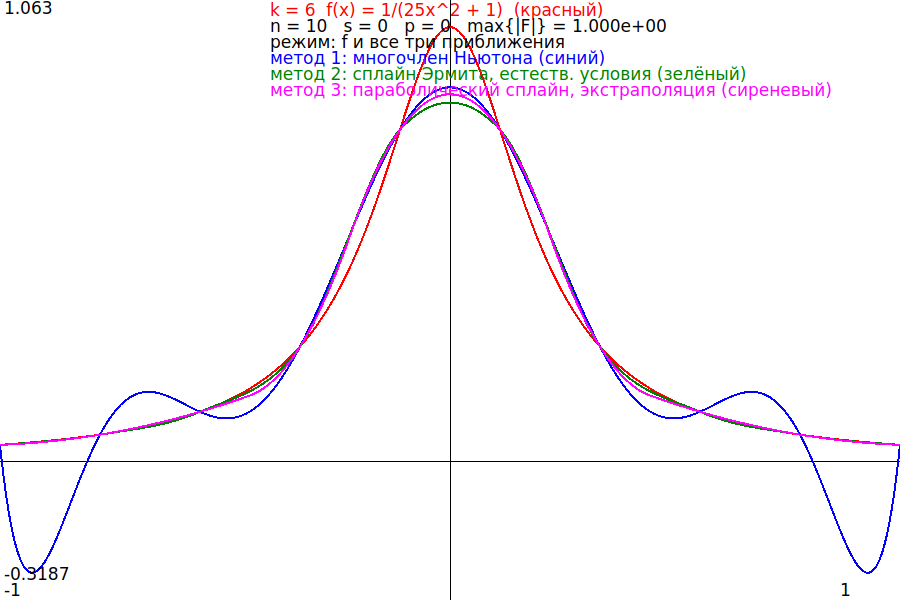
\includegraphics[width=0.85\textwidth]{../task2_yarik/screenshot_graphs.png}
\caption{Режим 4: функция Рунге $1/(25x^2+1)$ и все три приближения при $n=10$.
Красный~--- $f$, синий~--- многочлен Ньютона (хорошо видны колебания у краёв~---
эффект Рунге), зелёный~--- сплайн Эрмита, сиреневый~--- параболический сплайн.}
\end{figure}

\begin{figure}[h!]
\centering
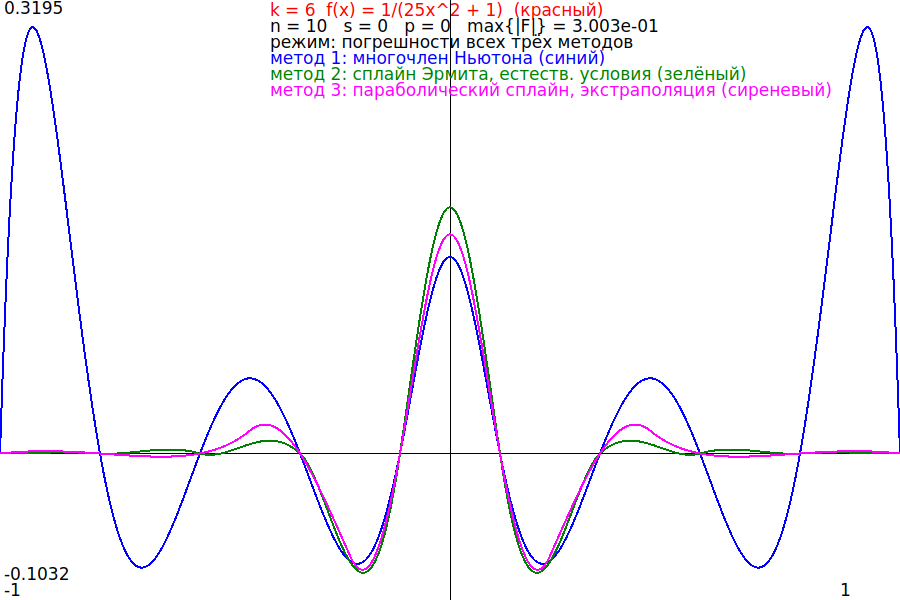
\includegraphics[width=0.85\textwidth]{../task2_yarik/screenshot_errors.png}
\caption{Режим 8: погрешности всех трёх методов для той же функции.
У многочлена Ньютона погрешность распределена по всему отрезку и растёт к краям,
у кусочных методов сосредоточена там, где функция плохо приближается~--- у пика.}
\end{figure}

\clearpage

\section{Проверки: что реально получилось}

\paragraph{Точность на многочленах} ($[-1,1]$, $n=5$, максимум модуля
погрешности по $5001$ точке):
\begin{center}
\begin{tabular}{lccc}
\toprule
$f$ & Ньютон & Эрмит (13) & Параболический (46) \\
\midrule
$1$   & $0$ & $0$ & $1{,}1\cdot10^{-16}$\\
$x$   & $0$ & $0$ & $1{,}1\cdot10^{-16}$\\
$x^2$ & $1{,}6\cdot10^{-16}$ & $1{,}9\cdot10^{-2}$ & $1{,}1\cdot10^{-16}$\\
$x^3$ & $2{,}4\cdot10^{-16}$ & $7{,}5\cdot10^{-2}$ & $4{,}3\cdot10^{-2}$\\
$x^4$ & $6{,}7\cdot10^{-16}$ & $1{,}4\cdot10^{-1}$ & $1{,}0\cdot10^{-1}$\\
\bottomrule
\end{tabular}
\end{center}
Многочлен Ньютона по пяти узлам точен на многочленах до четвёртой степени;
параболический сплайн с экстраполяцией~--- до второй; сплайн Эрмита с
естественными условиями~--- до первой.

\paragraph{Порядок сходимости}, $f=\dfrac{1}{25x^2+1}$, $[-1,1]$:
\begin{center}
\begin{tabular}{lcccc}
\toprule
$n$ & Эрмит & отношение & Параболический & отношение \\
\midrule
50   & $8{,}83\cdot10^{-4}$ & ---  & $4{,}02\cdot10^{-4}$ & --- \\
100  & $8{,}19\cdot10^{-5}$ & 10,8 & $4{,}05\cdot10^{-5}$ & 9,9 \\
200  & $9{,}57\cdot10^{-6}$ & 8,6  & $4{,}81\cdot10^{-6}$ & 8,4 \\
400  & $1{,}18\cdot10^{-6}$ & 8,1  & $5{,}91\cdot10^{-7}$ & 8,1 \\
800  & $1{,}47\cdot10^{-7}$ & 8,1  & $7{,}34\cdot10^{-8}$ & 8,1 \\
1600 & $1{,}83\cdot10^{-8}$ & 8,0  & $9{,}15\cdot10^{-9}$ & 8,0 \\
3200 & $2{,}29\cdot10^{-9}$ & 8,0  & $1{,}14\cdot10^{-9}$ & 8,0 \\
\bottomrule
\end{tabular}
\end{center}
Отношение $8$ при удвоении $n$ означает $O(h^3)$.

\paragraph{Тот же опыт для $f=e^{x}$ на $[0,1]$:}
\begin{center}
\begin{tabular}{lcccc}
\toprule
$n$ & Эрмит & отношение & Параболический & отношение \\
\midrule
50   & $4{,}25\cdot10^{-5}$ & --- & $1{,}31\cdot10^{-6}$ & --- \\
100  & $1{,}03\cdot10^{-5}$ & 4,1 & $1{,}60\cdot10^{-7}$ & 8,2 \\
200  & $2{,}55\cdot10^{-6}$ & 4,1 & $1{,}98\cdot10^{-8}$ & 8,1 \\
400  & $6{,}33\cdot10^{-7}$ & 4,0 & $2{,}46\cdot10^{-9}$ & 8,1 \\
800  & $1{,}58\cdot10^{-7}$ & 4,0 & $2{,}99\cdot10^{-10}$& 8,2 \\
1600 & $3{,}93\cdot10^{-8}$ & 4,0 & $3{,}74\cdot10^{-11}$& 8,0 \\
\bottomrule
\end{tabular}
\end{center}
У метода Эрмита максимум погрешности здесь достигается в приграничном отрезке,
где порядок $O(h^2)$~--- отсюда отношение $4$. У параболического сплайна
экстраполяционные граничные условия порядок не портят.

\paragraph{Скорость при $n=10^7$} ($[-1,1]$, $f=1/(25x^2+1)$):
построение сетки $0{,}16$~с, построение сплайна Эрмита $0{,}45$~с,
параболического $0{,}63$~с, вычисление $1200$ точек двух графиков
$0{,}0015$~с. Максимальная погрешность обоих методов при таком $n$ равна
$2\cdot10^{-16}$ и $4\cdot10^{-16}$~--- машинная точность.

\section{Вопросы, которые обычно задают}

\begin{description}
\item[Почему многочлен Ньютона, а не Лагранжа?] Это один и тот же многочлен,
разные формы записи. Форма Ньютона удобнее: добавление узла не требует
пересчёта, коэффициенты считаются за $O(n^2)$ и хранятся, а значение~--- за
$O(n)$ по схеме Горнера.

\item[Почему при $n>50$ многочлен не строится?] Из-за эффекта Рунге на
равномерной сетке приближение при больших $n$ не улучшается, а разваливается;
плюс стоимость $O(n^2)$. Это прямое требование задания.

\item[Точен ли метод~13 на параболе?] Нет, и это принципиально: естественные
условия требуют $S''=0$ на концах, а у параболы вторая производная постоянна и
отлична от нуля. Точность~--- только на многочленах степени $\le1$, зато метод
полностью локальный.

\item[Почему у метода~13 отношение погрешностей то $8$, то $4$?] Внутри
отрезка порядок $O(h^3)$, в двух приграничных отрезках~--- $O(h^2)$. Какое из
двух чисел окажется максимумом, зависит от функции, поэтому на $1/(25x^2+1)$
видно $8$, а на $e^x$~--- $4$.

\item[Зачем в задаче~46 точки склейки между узлами?] Иначе система
переопределена: $3n$ неизвестных и $3n$ условий плюс два граничных. Смещение
склеек на полшага даёт ровно две недостающие степени свободы.

\item[Почему прогонка без выбора главного элемента?] Матрица системы строго
диагонально доминирующая ($1,6,1$ на равномерной сетке), поэтому все
$|\alpha_i|<1$ и схема устойчива.

\item[Что происходит при нажатии клавиши~6 (возмущение)?] Значение в средней
точке заменяется на $f(x_{n/2})+p\cdot0{,}1\max|f|$, и все приближения строятся
заново по испорченным данным. Хорошо видно принципиальное различие: многочлен
Ньютона размазывает одну ошибку по всему отрезку, а кусочные методы
локализуют её в нескольких соседних отрезках.

\item[Почему при $n=10^7$ всё быстро?] Построение обоих кусочных методов
линейно по $n$, а рисование требует лишь по одной точке на пиксель, и каждая
стоит $O(\log n)$ (двоичный поиск отрезка).
\end{description}

\chapter{Задание 3. Интерполяция функции двух переменных по формуле Ньютона}
\label{ch:task3}

\section{Постановка}

Дана функция $f(x,y)$ на прямоугольнике $[a,b]\times[c,d]$ и сетка узлов
$x_1,\dots,x_{n_x}$ по первой переменной, $y_1,\dots,y_{n_y}$~--- по второй.
Нужно построить интерполяционный многочлен по формуле Ньютона (в двумерном
случае это интерполяция \emph{тензорными произведениями}) и показать в окне три
поверхности: саму функцию, приближение и погрешность.

Набор приближаемых функций:
\[
\begin{array}{llll}
k=0:\,1, & k=1:\,x, & k=2:\,y, & k=3:\,x+y,\\[2pt]
k=4:\,\sqrt{x^2+y^2}, & k=5:\,x^2+y^2, & k=6:\,e^{x^2-y^2}, &
k=7:\,\dfrac{1}{25(x^2+y^2)+1}.
\end{array}
\]
Запуск: \texttt{./graph3d a b c d nx ny mx my k}, где $n_x,n_y$~--- узлы
интерполяции, $m_x,m_y$~--- сетка триангуляции, по которой рисуется
поверхность (на само приближение она не влияет).

\section{Математика: тензорные произведения}

\subsection{Базис}

Как в конспекте (§1.5.3), берём одномерные базисы Ньютона по каждой переменной:
\[
u_i(x)=\prod_{k=1}^{i-1}(x-x_k),\quad i=1,\dots,n_x,\qquad
v_j(y)=\prod_{l=1}^{j-1}(y-y_l),\quad j=1,\dots,n_y
\]
(пустое произведение равно единице, так что $u_1\equiv v_1\equiv1$). Базис в
пространстве функций двух переменных~--- тензорные произведения
\[
w_{ij}(x,y)=u_i(x)\,v_j(y)=\prod_{k=1}^{i-1}\prod_{l=1}^{j-1}(x-x_k)(y-y_l),
\]
а приближающая функция ищется в виде
\[
P(x,y)=\sum_{i=1}^{n_x}\sum_{j=1}^{n_y}c_{ij}\,u_i(x)\,v_j(y).
\]
Функционалы~--- значения в узлах; матрицы $A$ и $B$ из общей схемы единичные,
поэтому коэффициенты равны смешанным (двойным) разделённым разностям
\[
c_{ij}=f[x_1,\dots,x_i;\,y_1,\dots,y_j].
\]
Смешанная разделённая разность~--- это обычная разделённая разность по $x$,
применённая к разделённой разности по $y$ (и наоборот: порядок не важен, так
как обе операции линейны и действуют по разным индексам).

\subsection{Почему это действительно интерполяция}

\begin{utv}
$P(x_l,y_m)=f(x_l,y_m)$ для всех $l=1,\dots,n_x$, $m=1,\dots,n_y$.
\end{utv}
\begin{proof}
Перепишем сумму как
$P(x,y)=\sum_i u_i(x)\,g_i(y)$, где
$g_i(y)=\sum_j f[x_1,\dots,x_i;y_1,\dots,y_j]\,v_j(y)$.
При фиксированном $i$ выражение $g_i$~--- это одномерный интерполяционный
многочлен Ньютона (по переменной $y$) для функции
$y\mapsto f[x_1,\dots,x_i;\,y]$, то есть для разделённой разности по $x$,
рассматриваемой как функция $y$. По одномерной теореме об интерполяции
$g_i(y_m)=f[x_1,\dots,x_i;\,y_m]$ для всех $m$.

Теперь при фиксированном $m$ функция
$x\mapsto P(x,y_m)=\sum_i u_i(x)\,f[x_1,\dots,x_i;y_m]$~--- это одномерный
многочлен Ньютона для функции $x\mapsto f(x,y_m)$, а значит,
$P(x_l,y_m)=f(x_l,y_m)$.
\end{proof}

\begin{utv}
Если $f$~--- многочлен степени $\le n_x-1$ по $x$ и $\le n_y-1$ по $y$, то
$P\equiv f$.
\end{utv}
\begin{proof}
Оба одномерных шага в доказательстве выше точны на многочленах
соответствующих степеней.
\end{proof}

\subsection{Алгоритм: два прохода по таблице}

Коэффициенты считаются прямо в массиве, в два прохода.

\textbf{Шаг 0.} $c_{ij}=f(x_i,y_j)$.

\textbf{Шаг 1 (по $x$).} Для $\text{level}=1,\dots,n_x-1$ и для
$i=n_x-1$ вниз до $\text{level}$:
\[
c_{ij}\;\leftarrow\;\frac{c_{ij}-c_{i-1,j}}{x_i-x_{i-\text{level}}}
\qquad\text{сразу для всех } j .
\]
После этого в строке $i$ стоят разделённые разности по $x$ порядка $i-1$.

\textbf{Шаг 2 (по $y$).} То же самое внутри каждой строки:
для $\text{level}=1,\dots,n_y-1$ и $j=n_y-1$ вниз до $\text{level}$:
\[
c_{ij}\;\leftarrow\;\frac{c_{ij}-c_{i,j-1}}{y_j-y_{j-\text{level}}} .
\]

Движение «сверху вниз» по индексу (от большого к меньшему) нужно ровно по той
же причине, что и в одномерном случае: значение $c_{i-1,j}$ ещё понадобится.
Сложность: $O(n_x^2n_y+n_xn_y^2)$ действий и $O(n_xn_y)$ памяти
(дополнительной памяти нет вовсе, всё делается на месте).

Соответствующий код:
\begin{lstlisting}[style=cpp]
for (int level = 1; level < nx; level++)
    for (int i = nx - 1; i >= level; i--) {
        dx = x_nodes[i] - x_nodes[i - level];
        for (int j = 0; j < ny; j++)
            coeffs[i*ny + j] = (coeffs[i*ny + j] - coeffs[(i-1)*ny + j]) / dx;
    }
for (int i = 0; i < nx; i++)
    for (int level = 1; level < ny; level++)
        for (int j = ny - 1; j >= level; j--) {
            dy = y_nodes[j] - y_nodes[j - level];
            coeffs[i*ny + j] = (coeffs[i*ny + j] - coeffs[i*ny + (j-1)]) / dy;
        }
\end{lstlisting}
Обратите внимание на порядок циклов в первом проходе: внутренний цикл по $j$
идёт по подряд лежащей памяти (хранение построчное,
\texttt{f[i*ny+j]}), поэтому кэш используется эффективно.

\subsection{Вычисление значения: двойная схема Горнера}

\[
P(x,y)=g_1(y)+(x-x_1)\Bigl(g_2(y)+(x-x_2)\bigl(\dots\bigr)\Bigr),\qquad
g_i(y)=c_{i1}+(y-y_1)\bigl(c_{i2}+(y-y_2)(\dots)\bigr).
\]
\begin{lstlisting}[style=cpp]
result = coeffs[(nx-1)*ny + ny-1];
for (int j = ny - 2; j >= 0; j--)
    result = result * (py - y_nodes[j]) + coeffs[(nx-1)*ny + j];
for (int i = nx - 2; i >= 0; i--) {
    inner = coeffs[i*ny + ny-1];
    for (int j = ny - 2; j >= 0; j--)
        inner = inner * (py - y_nodes[j]) + coeffs[i*ny + j];
    result = result * (px - x_nodes[i]) + inner;
}
\end{lstlisting}
Стоимость $O(n_xn_y)$ на одну точку; произведения $u_i(x)$, $v_j(y)$ явно
не вычисляются.

\section{Выбор узлов: Чебышёв и порядок Лежа}

\subsection{Почему не равномерные узлы}

В двумерном случае эффект Рунге никуда не девается (он есть уже по каждой
переменной). Поэтому узлы берутся чебышёвские~--- нули многочлена Чебышёва:
\[
t_i=\frac{a+b}{2}+\frac{b-a}{2}\cos\frac{\pi(i+\tfrac12)}{n},\qquad i=0,\dots,n-1 .
\]
Для них величина $\max|\omega(x)|$ минимальна среди всех расположений узлов, и
интерполяция ведёт себя хорошо. Проверка (функция
$1/(25(x^2+y^2)+1)$, $n_x=n_y=30$, максимум погрешности по сетке $150\times150$):
\begin{center}
\begin{tabular}{ll}
\toprule
равномерные узлы & $1{,}77\cdot10^{6}$ \\
узлы Чебышёва & $9{,}93\cdot10^{-3}$ \\
\bottomrule
\end{tabular}
\end{center}

\subsection{Почему важен порядок узлов (тонкое место)}

Сам многочлен от порядка узлов не зависит~--- он единственный. Но \emph{схема
вычислений} зависит: разделённые разности высокого порядка при монотонном
(по возрастанию) порядке узлов содержат огромные взаимно сокращающиеся
слагаемые, и ошибки округления растут лавинообразно. Лечение~--- перестановка
узлов в последовательность Лежа: очередным берётся узел, максимизирующий
произведение расстояний до уже выбранных,
\[
t_{k}=\arg\max_{t}\prod_{m<k}|t-t_m| .
\]
Реализуется за $O(n^2)$ с инкрементальным пересчётом весов:
\begin{lstlisting}[style=cpp]
for (int i = 0; i < n; i++) weight[i] = fabs(nodes[i] - center);
for (int k = 0; k < n - 1; k++) {
    /* pick the largest weight among the rest and swap it into position k */
    for (int i = k + 1; i < n; i++)
        weight[i] *= fabs(nodes[i] - nodes[k]);
}
\end{lstlisting}
Что это даёт (максимум $|f-P|$, узлы Чебышёва, $[-1,1]^2$):
\begin{center}
\begin{tabular}{lcc|cc}
\toprule
& \multicolumn{2}{c|}{$f=e^{x^2-y^2}$} & \multicolumn{2}{c}{$f=1/(25(x^2+y^2)+1)$}\\
$n$ & монотонный & Лежа & монотонный & Лежа\\
\midrule
16 & $2{,}66\cdot10^{-9}$ & $2{,}66\cdot10^{-9}$ & $1{,}42\cdot10^{-1}$ & $1{,}42\cdot10^{-1}$\\
24 & $2{,}33\cdot10^{-13}$& $2{,}22\cdot10^{-15}$& --- & ---\\
32 & $2{,}49\cdot10^{-5}$ & $2{,}22\cdot10^{-15}$& $7{,}97\cdot10^{1}$ & $6{,}72\cdot10^{-3}$\\
40 & $1{,}33\cdot10^{3}$  & $2{,}22\cdot10^{-15}$& $1{,}86\cdot10^{6}$ & $1{,}39\cdot10^{-3}$\\
50 & $2{,}47\cdot10^{13}$ & $3{,}77\cdot10^{-15}$& $8{,}11\cdot10^{11}$& $1{,}93\cdot10^{-4}$\\
64 & $5{,}23\cdot10^{27}$ & $5{,}55\cdot10^{-15}$& $1{,}73\cdot10^{25}$& $1{,}20\cdot10^{-5}$\\
\bottomrule
\end{tabular}
\end{center}
Без перестановки программа при $n_x=n_y=32$ уже рисует мусор; с
перестановкой всё остаётся на уровне машинной точности. Это хороший ответ на
вопрос «а почему у вас узлы лежат в странном порядке».

\section{Трёхмерная графика без OpenGL}

\subsection{Что рисуется}

Поверхность $z=F(x,y)$, где $F$~--- либо $f$, либо $P$, либо $f-P$
(переключается клавишей~1). Область разбивается сеткой $m_x\times m_y$ точек;
в каждой считается значение, попутно находятся $\min z$ и $\max z$ и
выводится $\max\{|F|\}$.

\subsection{Нормировка и проекция}

Координаты приводятся к кубу $[-1,1]^3$:
\[
\tilde x=\frac{x-c_x}{h_x},\quad
\tilde y=\frac{y-c_y}{h_y},\quad
\tilde z=0{,}8\Bigl(2\frac{z-z_{\min}}{z_{\max}-z_{\min}}-1\Bigr),
\]
где $c_x,h_x$~--- центр и полуширина отображаемого прямоугольника. Благодаря
этому картинка никогда не выходит за окно и никогда не оказывается слишком
мелкой, а масштабы по осям независимы.

Камера задаётся двумя углами: $\varphi$~--- поворот вокруг вертикальной оси
(клавиши 8 и 9), $\theta$~--- подъём над плоскостью (клавиши Up/Down). Орты
системы координат наблюдателя:
\[
\mathbf r=(-\sin\varphi,\ \cos\varphi,\ 0),\qquad
\mathbf u=(-\sin\theta\cos\varphi,\ -\sin\theta\sin\varphi,\ \cos\theta),\qquad
\mathbf n=(\cos\theta\cos\varphi,\ \cos\theta\sin\varphi,\ \sin\theta).
\]
Легко проверить, что тройка $(\mathbf r,\mathbf u,\mathbf n)$ ортонормирована.
Экранные координаты точки $\mathbf p$~--- это скалярные произведения
$(\mathbf p,\mathbf r)$ и $(\mathbf p,\mathbf u)$, а глубина~---
$(\mathbf p,\mathbf n)$: чем больше, тем ближе к наблюдателю. Проекция
ортогональная (параллельная), поэтому прямоугольная сетка остаётся сеткой и
картинка читается лучше, чем при перспективе.
\begin{lstlisting}[style=cpp]
sx = -nX*sin(phi) + nY*cos(phi);
sy = -(nX*cos(phi) + nY*sin(phi))*sin(theta) + nZ*cos(theta);
depth = (nX*cos(phi) + nY*sin(phi))*cos(theta) + nZ*sin(theta);
scale = 0.32*min(width(), height());
return QPointF(0.5*width() + scale*sx, 0.55*height() - scale*sy);
\end{lstlisting}

\subsection{Видимость: алгоритм художника}

Задача «что кого закрывает» решается самым простым надёжным способом: все
клетки сетки сортируются по глубине своего центра и рисуются от дальних к
ближним, ближние закрывают дальние. Для графика функции (каждой точке $(x,y)$
отвечает ровно одно $z$) этого достаточно~--- взаимных пересечений у клеток
нет. Стоимость кадра $O(m_xm_y\log(m_xm_y))$.

Цвет клетки зависит от её средней высоты: синий $\to$ голубой $\to$ зелёный
$\to$ жёлтый $\to$ красный. При небольших сетках дополнительно рисуются рёбра,
при больших они отключаются, иначе картинка превращается в сплошную сетку.

\section{Разбор программы}

\begin{center}
\begin{tabular}{ll}
\toprule
Файл & Содержимое \\
\midrule
\texttt{functions2d.cpp/.h} & восемь функций $f(x,y)$ и их описания \\
\texttt{newton2d.cpp/.h} & узлы, порядок Лежа, коэффициенты, значение, погрешность \\
\texttt{window3d.cpp/.h} & сетка, проекция, рисование, клавиши \\
\texttt{main.cpp} & аргументы, окно, меню, строка состояния \\
\texttt{graph3d.pro} & проект для qmake \\
\bottomrule
\end{tabular}
\end{center}

Ключевые функции метода:
\begin{lstlisting}[style=cpp]
void   make_chebyshev_nodes(int n, double a, double b, double *nodes);
void   reorder_nodes_leja(int n, double *nodes);
int    make_newton2d_coefficients(int nx, int ny, const double *x, const double *y,
                                  const double *f, double *coeffs);
double calculate_newton2d_value(double px, double py, int nx, int ny,
                                const double *x, const double *y, const double *coeffs);
double calculate_newton2d_discrepancy(double px, double py, func2_t func, int nx, int ny,
                                      const double *x, const double *y, const double *coeffs);
\end{lstlisting}
Значения и коэффициенты хранятся построчно: \texttt{f[i*ny+j]} отвечает узлу
$(x_i,y_j)$. Возмущение (клавиши 6 и 7) добавляется к значению в центральном
узле, после чего коэффициенты строятся заново.

Виджет \texttt{Window3D} делает три вещи: \texttt{build\_interpolation()}
(узлы $\to$ порядок Лежа $\to$ значения $\to$ коэффициенты),
\texttt{build\_mesh()} (значения на сетке рисования, $\min z$, $\max z$,
$\max|F|$) и \texttt{paintEvent()} (каркас, поверхность, надписи). Каждое
нажатие клавиши вызывает ровно те этапы, которые действительно изменились:
смена режима не пересчитывает коэффициенты, поворот камеры не пересчитывает
даже сетку.

\section{Как это выглядит}

\begin{figure}[h!]
\centering
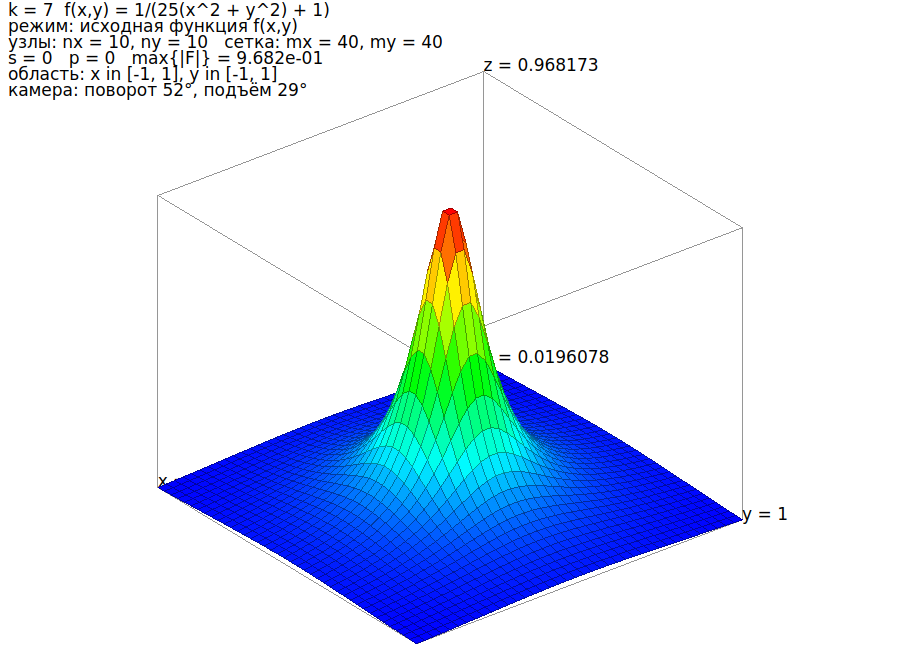
\includegraphics[width=0.78\textwidth]{../task3_yarik/screenshot_function.png}
\caption{Режим «функция»: $f(x,y)=1/(25(x^2+y^2)+1)$ на $[-1,1]^2$.
В левом верхнем углу~--- вся служебная информация: номер функции, режим,
$n_x,n_y$, $m_x,m_y$, масштаб, возмущение, $\max|F|$ и углы камеры.}
\end{figure}

\begin{figure}[h!]
\centering
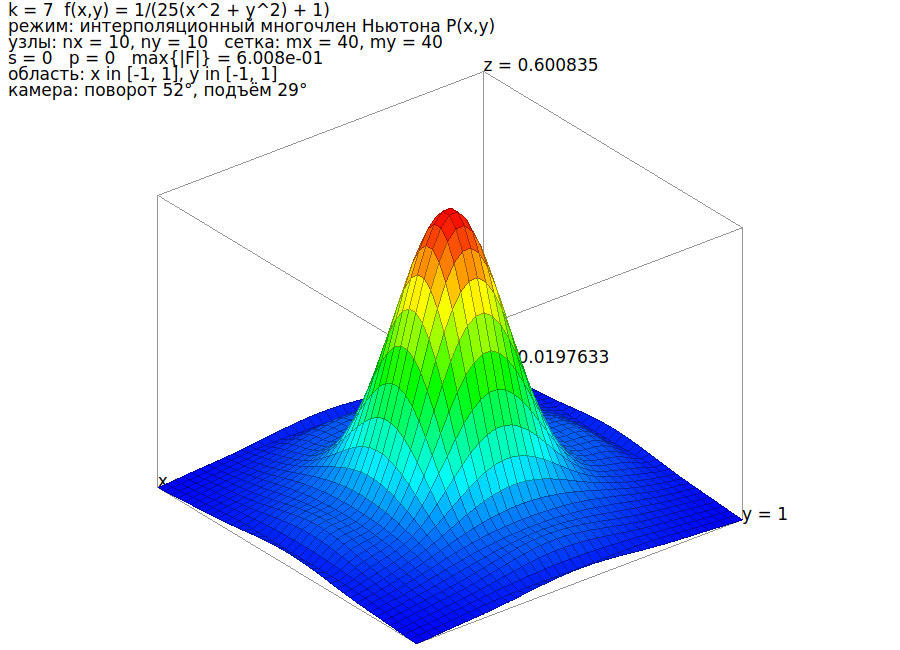
\includegraphics[width=0.78\textwidth]{../task3_yarik/screenshot_newton.png}
\caption{Режим «приближение»: интерполяционный многочлен Ньютона по сетке
$10\times10$ узлов. Пик занижен~--- десяти узлов на такую функцию не хватает.}
\end{figure}

\begin{figure}[h!]
\centering
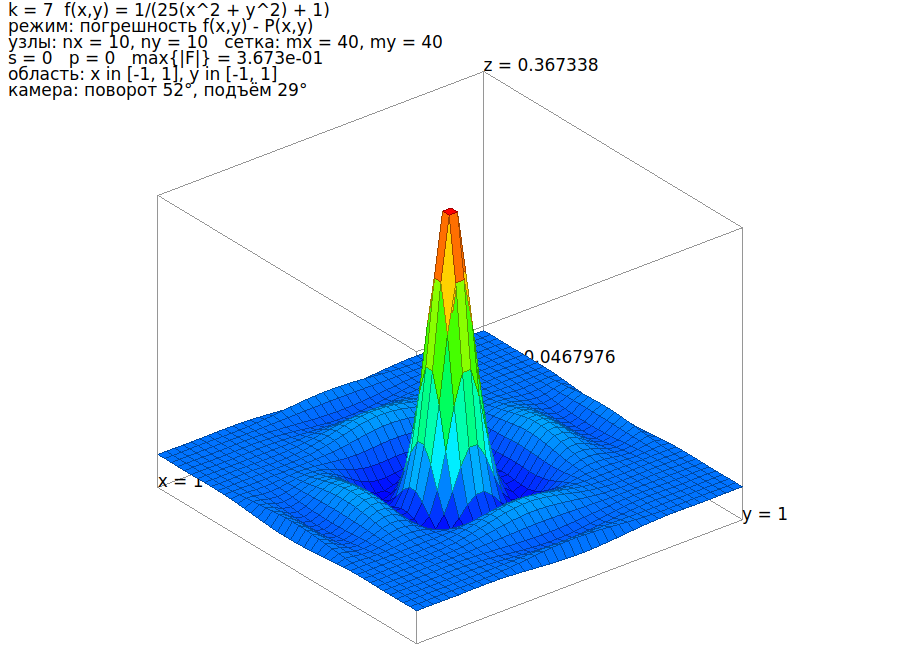
\includegraphics[width=0.78\textwidth]{../task3_yarik/screenshot_error.png}
\caption{Режим «погрешность» $f-P$: максимум ошибки сидит ровно на пике,
по краям области поверхность почти плоская.}
\end{figure}

\clearpage

\section{Проверки: что реально получилось}

\paragraph{1. Интерполяция точна в узлах.} Для всех восьми функций при
$n_x=n_y=5$ максимум $|P(x_i,y_j)-f(x_i,y_j)|$ по всем узлам не превосходит
$10^{-15}$.

\paragraph{2. Точность на многочленах} ($[-1,1]^2$, $n_x=n_y=5$, максимум по
сетке $120\times120$):
\begin{center}
\begin{tabular}{ll}
\toprule
$f$ & $\max|f-P|$ \\
\midrule
$1$ & $0$ \\
$x$ & $1{,}1\cdot10^{-16}$ \\
$y$ & $1{,}1\cdot10^{-16}$ \\
$x+y$ & $4{,}4\cdot10^{-16}$ \\
$x^2+y^2$ & $8{,}9\cdot10^{-16}$ \\
$\sqrt{x^2+y^2}$ & $1{,}3\cdot10^{-1}$ (негладкая в нуле) \\
$e^{x^2-y^2}$ & $2{,}4\cdot10^{-2}$ \\
$1/(25(x^2+y^2)+1)$ & $4{,}1\cdot10^{-1}$ \\
\bottomrule
\end{tabular}
\end{center}

\paragraph{3. Сходимость} ($[-1,1]^2$, узлы Чебышёва в порядке Лежа):
\begin{center}
\begin{tabular}{lcc}
\toprule
$n=n_x=n_y$ & $e^{x^2-y^2}$ & $1/(25(x^2+y^2)+1)$ \\
\midrule
4  & $2{,}42\cdot10^{-1}$ & $8{,}43\cdot10^{-1}$\\
8  & $1{,}20\cdot10^{-3}$ & $5{,}31\cdot10^{-1}$\\
16 & $2{,}66\cdot10^{-9}$ & $1{,}42\cdot10^{-1}$\\
32 & $2{,}66\cdot10^{-15}$& $6{,}72\cdot10^{-3}$\\
50 & $2{,}89\cdot10^{-15}$& $1{,}93\cdot10^{-4}$\\
\bottomrule
\end{tabular}
\end{center}
Для аналитической функции сходимость экспоненциальная~--- машинная точность уже
при 32 узлах. Для функции с «пиком» сходимость медленнее, но она есть
(на равномерных узлах её бы не было вовсе).

\paragraph{4. Скорость.} Самый тяжёлый режим ($n_x=n_y=64$, сетка
$128\times128$): построение коэффициентов~--- меньше $1$~мс, полный пересчёт
поверхности (16\,384 точки по $O(n_xn_y)$ каждая)~--- $0{,}22$~с, отрисовка
кадра~--- $0{,}04$~с.

\paragraph{5. Устойчивость интерфейса.} Прогон, в котором для всех восьми
функций последовательно нажимаются все клавиши (режимы, узлы, сетка, масштаб,
возмущение, повороты)~--- около 400 перестроений~--- проходит без падений, без
NaN и без зависаний.

\section{Вопросы, которые обычно задают}

\begin{description}
\item[Почему это «формула Ньютона», а не просто двумерная интерполяция?]
Потому что базис и коэффициенты~--- ньютоновские по каждой переменной:
$w_{ij}=u_iv_j$, $c_{ij}=f[x_1..x_i;y_1..y_j]$. Это буквально тензорное
произведение двух одномерных формул Ньютона.

\item[Важен ли порядок проходов (сначала по $x$, потом по $y$)?] Нет. Обе
операции линейны и действуют по разным индексам, поэтому коммутируют; результат
одинаков.

\item[Какова степень получающегося многочлена?] Не выше $n_x-1$ по $x$ и
$n_y-1$ по $y$; полная степень может достигать $n_x+n_y-2$. Он точен на всех
таких многочленах.

\item[Почему нельзя взять равномерные узлы?] Эффект Рунге: при
$n_x=n_y=30$ погрешность на равномерных узлах $\sim10^{6}$ против
$10^{-2}$ на чебышёвских.

\item[Зачем перестановка Лежа?] Это чисто вычислительный приём: он не меняет
многочлен, но делает вычисление разделённых разностей и схему Горнера
устойчивыми. Без него при $n\ge32$ результат разваливается (см. таблицу).

\item[Почему алгоритм художника, а не $z$-буфер?] Для графика функции клетки
не пересекаются, поэтому сортировки по глубине достаточно; это проще и не
требует памяти под буфер глубины.

\item[Что показывает режим погрешности при возмущении?] Что многочленная
интерполяция \emph{нелокальна}: испорченное значение в одном узле меняет
приближение по всей области. У кусочных методов (задание~2) такого нет.
\end{description}

\appendix

\chapter{Сборка: какие библиотеки нужны}

\section{Задание 1 (MPI)}
\begin{lstlisting}[style=c]
sudo apt install build-essential openmpi-bin libopenmpi-dev   # Ubuntu/Debian
brew install open-mpi                                          # macOS
\end{lstlisting}
Сборка:
\begin{lstlisting}[style=c]
cd task1_yarik
make                      # or, in a single command:
mpicc -O2 -Wall -Wextra main.c input.c output.c gauss_reverse_MPI.c -o a.out -lm
mpirun -np 4 ./a.out 1000 5 1
\end{lstlisting}

\section{Задания 2 и 3 (Qt)}
\begin{lstlisting}[style=c]
sudo apt install build-essential qtbase5-dev qtbase5-dev-tools qt5-qmake  # Qt5
sudo apt install build-essential qt6-base-dev qt6-base-dev-tools          # Qt6
brew install qt                                                           # macOS
\end{lstlisting}
Сборка и запуск:
\begin{lstlisting}[style=c]
cd task2_yarik && qmake graph.pro && make && ./graph -1 1 10 6
cd task3_yarik && qmake graph3d.pro && make && ./graph3d -1 1 -1 1 10 10 40 40 7
\end{lstlisting}
Если \texttt{qmake} не находится, он может называться \texttt{qmake6} или
\texttt{qmake-qt5}. Сборка без qmake (нужно самому вызвать \texttt{moc})
описана в файлах \texttt{разбор.txt} в каждой папке.

\chapter{Шпаргалка по клавишам}

\section{Задание 2}
\begin{center}
\begin{tabular}{ll}
\toprule
Клавиша & Действие \\
\midrule
0 & следующая функция $f_k$ (возмущение сбрасывается) \\
1 & следующий набор графиков (9 режимов) \\
2 / 3 & увеличить / уменьшить масштаб по $x$ вдвое \\
4 / 5 & удвоить / уменьшить вдвое число узлов $n$ \\
6 / 7 & увеличить / уменьшить возмущение $p$ \\
Ctrl+Q & выход \\
\bottomrule
\end{tabular}
\end{center}

\section{Задание 3}
\begin{center}
\begin{tabular}{ll}
\toprule
Клавиша & Действие \\
\midrule
0 & следующая функция $f_k$ \\
1 & режим: функция $\to$ приближение $\to$ погрешность \\
2 / 3 & увеличить / уменьшить масштаб области \\
4 / 5 & удвоить / уменьшить вдвое $n_x,n_y$ \\
6 / 7 & увеличить / уменьшить возмущение $p$ \\
8 / 9 & повернуть камеру влево / вправо \\
+ / -- & удвоить / уменьшить вдвое сетку рисования $m_x,m_y$ \\
Up / Down & поднять / опустить камеру \\
Ctrl+Q & выход \\
\bottomrule
\end{tabular}
\end{center}

\chapter{Частые ошибки и как их чинить}

\begin{description}
\item[\texttt{mpi.h: No such file or directory}] не установлен
\texttt{libopenmpi-dev}, либо сборка идёт через \texttt{gcc} вместо
\texttt{mpicc}.

\item[Программа на MPI работает медленнее на большем числе процессов]
процессов больше, чем физических ядер. Смотрите \texttt{nproc}; на двух ядрах
запуск с \texttt{-np 4} даёт замедление в несколько раз.

\item[\texttt{qmake: command not found}] в новых Ubuntu команда называется
\texttt{qmake6}; либо не установлен пакет \texttt{qt5-qmake}.

\item[Ошибки вида \texttt{undefined reference to `vtable for Window'}]
не запущен \texttt{moc} для заголовка с макросом \texttt{Q\_OBJECT}
(при сборке через qmake это делается автоматически).

\item[График «прыгает» при изменении размера окна] так и задумано: масштаб
по вертикали пересчитывается по реально видимым графикам, а число точек
выборки равно числу пикселей.

\item[При больших $n$ многочлен Ньютона не рисуется] это не ошибка:
при $n>50$ многочленное приближение по заданию не строится.
\end{description}

\chapter{Полные тексты файлов с методами}

Ниже приведены целиком те файлы, в которых живёт сама численная математика~---
именно о них чаще всего спрашивают на защите. Графические файлы
(\texttt{window.cpp}, \texttt{window3d.cpp}, \texttt{main.cpp}) разобраны в
тексте по частям, их полные версии лежат в репозитории.

\section{Задание 1: \texttt{gauss\_reverse\_MPI.c}}
\lstinputlisting[style=c,inputencoding=utf8/koi8-r]{../task1_yarik/gauss_reverse_MPI.c}

\section{Задание 1: \texttt{input.c}}
\lstinputlisting[style=c,inputencoding=utf8/koi8-r]{../task1_yarik/input.c}

\section{Задание 1: \texttt{output.c}}
\lstinputlisting[style=c,inputencoding=utf8/koi8-r]{../task1_yarik/output.c}

\section{Задание 1: \texttt{main.c}}
\lstinputlisting[style=c,inputencoding=utf8/koi8-r]{../task1_yarik/main.c}

\section{Задание 2: \texttt{newton\_interpolation.cpp}}
\lstinputlisting[style=cpp,inputencoding=utf8/koi8-r]{../task2_yarik/newton_interpolation.cpp}

\section{Задание 2: \texttt{hermite\_natural.cpp}}
\lstinputlisting[style=cpp,inputencoding=utf8/koi8-r]{../task2_yarik/hermite_natural.cpp}

\section{Задание 2: \texttt{parabolic\_extrapolation.cpp}}
\lstinputlisting[style=cpp,inputencoding=utf8/koi8-r]{../task2_yarik/parabolic_extrapolation.cpp}

\section{Задание 3: \texttt{newton2d.cpp}}
\lstinputlisting[style=cpp,inputencoding=utf8/koi8-r]{../task3_yarik/newton2d.cpp}

\end{document}
